\documentclass[11pt,a4paper,titlepage]{article}
\usepackage[utf8]{inputenc}
\usepackage{amsmath,amssymb,amsthm}
\usepackage[margin=1in]{geometry}
% References into Paper 1: its .aux is read under the name of this generation,
% the links go to the final name of its PDF
\usepackage{xr-hyper}
\externaldocument[P1-]{R_collatz_stop_at_the_drop_1}[R_collatz_stop_at_the_drop_1.pdf]
\usepackage{hyperref}
\hypersetup{colorlinks, allcolors=blue!50!black}
% Index: the entry of a key term links to the passage that introduces the term
\makeatletter
\newcommand{\termhere}[1]{\leavevmode
  \Hy@raisedlink{\hyper@anchorstart{term:#1}\hyper@anchorend}}
\newcommand{\boxhere}[1]{\leavevmode
  \Hy@raisedlink{\hyper@anchorstart{box:#1}\hyper@anchorend}}
\makeatother
\newcommand{\termlink}[2]{\hyperlink{term:#1}{#2}}
% A key term where it is introduced: italic, with a link to its entry in the box
% of its chapter (\boxhere)
\newcommand{\keyterm}[2]{\hyperlink{box:#1}{\emph{#2}}}
% A symbol that is a key term, where its meaning is given: the same link, no italics
\newcommand{\keysym}[2]{\hyperlink{box:#1}{#2}}
\usepackage{booktabs}
\usepackage{array}
\usepackage{xcolor}
\usepackage{tikz}
\definecolor{chordblue}{HTML}{2A78D6}
\definecolor{chordorange}{HTML}{EB6834}
\usepackage{etoolbox}
\IfFileExists{imakeidx.sty}
  {\usepackage{imakeidx}\makeindex[intoc]}
  {\usepackage{makeidx}\makeindex}

% Layout: paper (default) or screen: pdflatex "\def\screenversion{}\input{file}"
\newif\ifpaper
\papertrue
\ifdefined\screenversion \paperfalse \fi

% Lean declaration and pv.py command
\newcommand{\lean}[1]{\textsf{#1}}
\newcommand{\pv}[1]{\texttt{pv.py #1}}
% number in binary
\newcommand{\bin}[1]{\text{\texttt{#1}}_2}
\ExplSyntaxOn
\seq_new:N \l__bw_parts_seq
\bool_new:N \l__bw_first_bool
\cs_new_protected:Npn \__bw_part:n #1
  {
    \fcolorbox{black!50}{black!4}
      {
        \bool_set_true:N \l__bw_first_bool
        \tl_map_inline:nn {#1}
          {
            \bool_if:NF \l__bw_first_bool { \textcolor{black!30}{\vrule width 0.3pt} }
            \bool_set_false:N \l__bw_first_bool
            \makebox[0.62em]{\rule[-0.4ex]{0pt}{2.2ex}\ttfamily ##1}
          }
      }
  }
% binary word: digits in cells, parts split at "-"
\NewDocumentCommand \bw { m }
  {
    \text
      {
        \group_begin:
        \setlength{\fboxsep}{0pt}
        \setlength{\fboxrule}{0.4pt}
        \seq_set_split:Nnn \l__bw_parts_seq { - } {#1}
        \seq_map_indexed_inline:Nn \l__bw_parts_seq
          {
            \int_compare:nNnF {##1} = {1} { \hspace{0.1em}\texttt{-}\hspace{0.1em} }
            \__bw_part:n {##2}
          }
        \group_end:
      }
  }
\ExplSyntaxOff
% Words without frames: pdflatex "\def\plainwords{}\input{file}"
\ifdefined\plainwords \RenewDocumentCommand \bw { m } {\text{\texttt{#1}}} \fi
\usepackage{listings}
\lstset{basicstyle=\ttfamily\small, columns=fullflexible, keepspaces=true}

% Glossary box at the end of each chapter
\newsavebox{\wordboxbin}
\newenvironment{wordbox}
  {\par\ifpaper\vspace*{\fill}\vspace{\bigskipamount}\else\medskip\fi
   \noindent\begin{lrbox}{\wordboxbin}%
   \begin{minipage}{\dimexpr\linewidth-2\fboxsep-2\fboxrule\relax}\small
   \textbf{Key terms introduced in Chapter~\thesection:}\par\smallskip
   \begin{tabular}{@{}>{\bfseries\boldmath\raggedright\arraybackslash}p{0.24\linewidth}p{0.68\linewidth}@{}}}
  {\end{tabular}\end{minipage}\end{lrbox}%
   \fcolorbox{black!40}{black!3}{\usebox{\wordboxbin}}\par\ifpaper\else\medskip\fi}

% A figure or table set where it stands, on one page with what follows it
\makeatletter
\newenvironment{herefloat}[1]
  {\par\addvspace{\intextsep}\noindent\begin{minipage}{\linewidth}%
   \def\@captype{#1}\centering}
  {\end{minipage}\par\nopagebreak\vspace{\intextsep}}
\makeatother

\ifpaper\pretocmd{\section}{\clearpage}{}{}\fi
\newtheorem{theorem}{Theorem}
% the 3-smooth numbers up to 576 in increasing order, generated by smooth_fig.py
\newcommand{\smoothpath}{%
  \foreach \j in {0,...,9} \draw[darkgray, line width=0.3pt] (0.7125*\j,0) -- (0.7125*\j,-4.75);
  \foreach \i in {0,...,5} \draw[darkgray, line width=0.3pt] (0,-0.95*\i) -- (6.4125,-0.95*\i);
  \draw[chordblue, line width=0.7pt] (0.000,0.000) -- (0.713,0.000);
  \draw[chordorange, line width=0.7pt] (0.713,0.000) -- (0.000,-0.950);
  \draw[chordblue, line width=0.7pt] (0.000,-0.950) -- (1.425,0.000);
  \draw[chordorange, line width=0.7pt] (1.425,0.000) -- (0.713,-0.950);
  \draw[chordblue, line width=0.7pt] (0.713,-0.950) -- (2.138,0.000);
  \draw[chordorange, line width=0.7pt] (2.138,0.000) -- (0.000,-1.900);
  \draw[chordblue, line width=0.7pt] (0.000,-1.900) -- (1.425,-0.950);
  \draw[chordblue, line width=0.7pt] (1.425,-0.950) -- (2.850,0.000);
  \draw[chordorange, line width=0.7pt] (2.850,0.000) -- (0.713,-1.900);
  \draw[chordblue, line width=0.7pt] (0.713,-1.900) -- (2.138,-0.950);
  \draw[chordorange, line width=0.7pt] (2.138,-0.950) -- (0.000,-2.850);
  \draw[chordblue, line width=0.7pt] (0.000,-2.850) -- (3.562,0.000);
  \draw[chordorange, line width=0.7pt] (3.562,0.000) -- (1.425,-1.900);
  \draw[chordblue, line width=0.7pt] (1.425,-1.900) -- (2.850,-0.950);
  \draw[chordorange, line width=0.7pt] (2.850,-0.950) -- (0.713,-2.850);
  \draw[chordblue, line width=0.7pt] (0.713,-2.850) -- (4.275,0.000);
  \draw[chordorange, line width=0.7pt] (4.275,0.000) -- (2.138,-1.900);
  \draw[chordorange, line width=0.7pt] (2.138,-1.900) -- (0.000,-3.800);
  \draw[chordblue, line width=0.7pt] (0.000,-3.800) -- (3.562,-0.950);
  \draw[chordorange, line width=0.7pt] (3.562,-0.950) -- (1.425,-2.850);
  \draw[chordblue, line width=0.7pt] (1.425,-2.850) -- (4.987,0.000);
  \draw[chordorange, line width=0.7pt] (4.987,0.000) -- (2.850,-1.900);
  \draw[chordorange, line width=0.7pt] (2.850,-1.900) -- (0.713,-3.800);
  \draw[chordblue, line width=0.7pt] (0.713,-3.800) -- (4.275,-0.950);
  \draw[chordorange, line width=0.7pt] (4.275,-0.950) -- (2.138,-2.850);
  \draw[chordorange, line width=0.7pt] (2.138,-2.850) -- (0.000,-4.750);
  \draw[chordblue, line width=0.7pt] (0.000,-4.750) -- (5.700,0.000);
  \draw[chordorange, line width=0.7pt] (5.700,0.000) -- (3.562,-1.900);
  \draw[chordorange, line width=0.7pt] (3.562,-1.900) -- (1.425,-3.800);
  \draw[chordblue, line width=0.7pt] (1.425,-3.800) -- (4.987,-0.950);
  \draw[chordorange, line width=0.7pt] (4.987,-0.950) -- (2.850,-2.850);
  \draw[chordorange, line width=0.7pt] (2.850,-2.850) -- (0.713,-4.750);
  \draw[chordblue, line width=0.7pt] (0.713,-4.750) -- (6.413,0.000);
  \draw[chordorange, line width=0.7pt] (6.413,0.000) -- (4.275,-1.900);
  \fill[black!70] (0.000,0.000) circle (1.3pt);
  \node[font=\tiny, fill=white, inner sep=1pt, anchor=south east] at (-0.020,0.040) {$1$};
  \fill[black!70] (0.713,0.000) circle (1.3pt);
  \node[font=\tiny, fill=white, inner sep=1pt, anchor=south east] at (0.693,0.040) {$2$};
  \fill[black!70] (0.000,-0.950) circle (1.3pt);
  \node[font=\tiny, fill=white, inner sep=1pt, anchor=south east] at (-0.020,-0.910) {$3$};
  \fill[black!70] (1.425,0.000) circle (1.3pt);
  \node[font=\tiny, fill=white, inner sep=1pt, anchor=south east] at (1.405,0.040) {$4$};
  \fill[black!70] (0.713,-0.950) circle (1.3pt);
  \node[font=\tiny, fill=white, inner sep=1pt, anchor=south east] at (0.693,-0.910) {$6$};
  \fill[black!70] (2.138,0.000) circle (1.3pt);
  \node[font=\tiny, fill=white, inner sep=1pt, anchor=south east] at (2.118,0.040) {$8$};
  \fill[black!70] (0.000,-1.900) circle (1.3pt);
  \node[font=\tiny, fill=white, inner sep=1pt, anchor=south east] at (-0.020,-1.860) {$9$};
  \fill[black!70] (1.425,-0.950) circle (1.3pt);
  \node[font=\tiny, fill=white, inner sep=1pt, anchor=south east] at (1.405,-0.910) {$12$};
  \fill[black!70] (2.850,0.000) circle (1.3pt);
  \node[font=\tiny, fill=white, inner sep=1pt, anchor=south east] at (2.830,0.040) {$16$};
  \fill[black!70] (0.713,-1.900) circle (1.3pt);
  \node[font=\tiny, fill=white, inner sep=1pt, anchor=south east] at (0.693,-1.860) {$18$};
  \fill[black!70] (2.138,-0.950) circle (1.3pt);
  \node[font=\tiny, fill=white, inner sep=1pt, anchor=south east] at (2.118,-0.910) {$24$};
  \fill[black!70] (0.000,-2.850) circle (1.3pt);
  \node[font=\tiny, fill=white, inner sep=1pt, anchor=south east] at (-0.020,-2.810) {$27$};
  \fill[black!70] (3.562,0.000) circle (1.3pt);
  \node[font=\tiny, fill=white, inner sep=1pt, anchor=south east] at (3.542,0.040) {$32$};
  \fill[black!70] (1.425,-1.900) circle (1.3pt);
  \node[font=\tiny, fill=white, inner sep=1pt, anchor=south east] at (1.405,-1.860) {$36$};
  \fill[black!70] (2.850,-0.950) circle (1.3pt);
  \node[font=\tiny, fill=white, inner sep=1pt, anchor=south east] at (2.830,-0.910) {$48$};
  \fill[black!70] (0.713,-2.850) circle (1.3pt);
  \node[font=\tiny, fill=white, inner sep=1pt, anchor=south east] at (0.693,-2.810) {$54$};
  \fill[black!70] (4.275,0.000) circle (1.3pt);
  \node[font=\tiny, fill=white, inner sep=1pt, anchor=south east] at (4.255,0.040) {$64$};
  \fill[black!70] (2.138,-1.900) circle (1.3pt);
  \node[font=\tiny, fill=white, inner sep=1pt, anchor=south east] at (2.118,-1.860) {$72$};
  \fill[black!70] (0.000,-3.800) circle (1.3pt);
  \node[font=\tiny, fill=white, inner sep=1pt, anchor=south east] at (-0.020,-3.760) {$81$};
  \fill[black!70] (3.562,-0.950) circle (1.3pt);
  \node[font=\tiny, fill=white, inner sep=1pt, anchor=south east] at (3.542,-0.910) {$96$};
  \fill[black!70] (1.425,-2.850) circle (1.3pt);
  \node[font=\tiny, fill=white, inner sep=1pt, anchor=south east] at (1.405,-2.810) {$108$};
  \fill[black!70] (4.987,0.000) circle (1.3pt);
  \node[font=\tiny, fill=white, inner sep=1pt, anchor=south east] at (4.968,0.040) {$128$};
  \fill[black!70] (2.850,-1.900) circle (1.3pt);
  \node[font=\tiny, fill=white, inner sep=1pt, anchor=south east] at (2.830,-1.860) {$144$};
  \fill[black!70] (0.713,-3.800) circle (1.3pt);
  \node[font=\tiny, fill=white, inner sep=1pt, anchor=south east] at (0.693,-3.760) {$162$};
  \fill[black!70] (4.275,-0.950) circle (1.3pt);
  \node[font=\tiny, fill=white, inner sep=1pt, anchor=south east] at (4.255,-0.910) {$192$};
  \fill[black!70] (2.138,-2.850) circle (1.3pt);
  \node[font=\tiny, fill=white, inner sep=1pt, anchor=south east] at (2.118,-2.810) {$216$};
  \fill[black!70] (0.000,-4.750) circle (1.3pt);
  \node[font=\tiny, fill=white, inner sep=1pt, anchor=south east] at (-0.020,-4.710) {$243$};
  \fill[black!70] (5.700,0.000) circle (1.3pt);
  \node[font=\tiny, fill=white, inner sep=1pt, anchor=south east] at (5.680,0.040) {$256$};
  \fill[black!70] (3.562,-1.900) circle (1.3pt);
  \node[font=\tiny, fill=white, inner sep=1pt, anchor=south east] at (3.542,-1.860) {$288$};
  \fill[black!70] (1.425,-3.800) circle (1.3pt);
  \node[font=\tiny, fill=white, inner sep=1pt, anchor=south east] at (1.405,-3.760) {$324$};
  \fill[black!70] (4.987,-0.950) circle (1.3pt);
  \node[font=\tiny, fill=white, inner sep=1pt, anchor=south east] at (4.968,-0.910) {$384$};
  \fill[black!70] (2.850,-2.850) circle (1.3pt);
  \node[font=\tiny, fill=white, inner sep=1pt, anchor=south east] at (2.830,-2.810) {$432$};
  \fill[black!70] (0.713,-4.750) circle (1.3pt);
  \node[font=\tiny, fill=white, inner sep=1pt, anchor=south east] at (0.693,-4.710) {$486$};
  \fill[black!70] (6.413,0.000) circle (1.3pt);
  \node[font=\tiny, fill=white, inner sep=1pt, anchor=south east] at (6.393,0.040) {$512$};
  \fill[black!70] (4.275,-1.900) circle (1.3pt);
  \node[font=\tiny, fill=white, inner sep=1pt, anchor=south east] at (4.255,-1.860) {$576$};
}
% drop grid of 39, generated by a throwaway script
\newcommand{\dropgridXXXIX}{%
  \draw[chordblue, fill=chordblue!35] (0.00,0.00) rectangle ++(1.25,-0.60);
  \node at (0.625,-0.300) {\small $39$};
  \draw[chordblue, fill=chordblue!35] (1.25,0.00) rectangle ++(1.25,-0.60);
  \node at (1.875,-0.300) {\small $59$};
  \draw[chordblue, fill=chordblue!35] (2.50,0.00) rectangle ++(1.25,-0.60);
  \node at (3.125,-0.300) {\small $89$};
  \draw[black!45, fill=white] (3.75,0.00) rectangle ++(1.25,-0.60);
  \node at (4.375,-0.300) {\small $134$};
  \draw[chordblue, fill=chordblue!35] (3.75,-0.60) rectangle ++(1.25,-0.60);
  \node at (4.375,-0.900) {\small $67$};
  \draw[chordblue, fill=chordblue!35] (5.00,0.00) rectangle ++(1.25,-0.60);
  \node at (5.625,-0.300) {\small $101$};
  \draw[black!45, fill=white] (6.25,0.00) rectangle ++(1.25,-0.60);
  \node at (6.875,-0.300) {\small $152$};
  \draw[black!45, fill=white] (6.25,-0.60) rectangle ++(1.25,-0.60);
  \node at (6.875,-0.900) {\small $76$};
  \draw[black!45, fill=black!6] (6.25,-1.20) rectangle ++(1.25,-0.60);
  \node at (6.875,-1.500) {\small $38$};
  \node at (0.625,-2.150) {\texttt{[}};
  \node at (1.875,-2.150) {\texttt{[}};
  \node at (3.125,-2.150) {\texttt{(}};
  \node at (4.375,-2.150) {\texttt{)[}};
  \node at (5.625,-2.150) {\texttt{\char123}};
  \node at (6.875,-2.150) {\texttt{\char125]]]}};
}
% Stern-Brocot path toward log2 3, generated by a throwaway script
\newcommand{\sternbrocotpath}{%
  \draw[black!45] (0.00,0.00) -- (0.55,-0.52);
  \draw[black!45] (0.55,-0.52) -- (0.00,-1.04);
  \draw[black!45] (0.00,-1.04) -- (0.55,-1.56);
  \draw[black!45] (0.55,-1.56) -- (0.00,-2.08);
  \draw[black!45] (0.00,-2.08) -- (-0.55,-2.60);
  \draw[black!45] (-0.55,-2.60) -- (0.00,-3.12);
  \draw[black!45] (0.00,-3.12) -- (0.55,-3.64);
  \draw[black!45] (0.55,-3.64) -- (0.00,-4.16);
  \draw[black!45] (0.00,-4.16) -- (-0.55,-4.68);
  \draw[black!45] (-0.55,-4.68) -- (-1.10,-5.20);
  \draw[black!45] (-1.10,-5.20) -- (-0.55,-5.72);
  \draw[black!45] (-0.55,-5.72) -- (-1.10,-6.24);
  \draw[black!45] (-1.10,-6.24) -- (-1.65,-6.76);
  \draw[black!45] (-1.65,-6.76) -- (-2.20,-7.28);
  \draw[black!45] (-2.20,-7.28) -- (-2.75,-7.80);
  \fill[chordorange] (0.00,0.00) circle (1.6pt);
  \node[left, font=\small, text=chordorange] at (0.00,0.00) {$\frac{1}{1}$};
  \fill[chordblue] (0.55,-0.52) circle (1.6pt);
  \node[right, font=\small, text=chordblue] at (0.55,-0.52) {$\frac{2}{1}$};
  \fill[chordorange] (0.00,-1.04) circle (1.6pt);
  \node[left, font=\small, text=chordorange] at (0.00,-1.04) {$\frac{3}{2}$};
  \fill[chordblue] (0.55,-1.56) circle (1.6pt);
  \node[right, font=\small, text=chordblue] at (0.55,-1.56) {$\frac{5}{3}$};
  \fill[chordblue] (0.00,-2.08) circle (1.6pt);
  \node[right, font=\small, text=chordblue] at (0.00,-2.08) {$\frac{8}{5}$};
  \fill[chordorange] (-0.55,-2.60) circle (1.6pt);
  \node[left, font=\small, text=chordorange] at (-0.55,-2.60) {$\frac{11}{7}$};
  \fill[chordorange] (0.00,-3.12) circle (1.6pt);
  \node[left, font=\small, text=chordorange] at (0.00,-3.12) {$\frac{19}{12}$};
  \fill[chordblue] (0.55,-3.64) circle (1.6pt);
  \node[right, font=\small, text=chordblue] at (0.55,-3.64) {$\frac{27}{17}$};
  \draw[chordblue, line width=0.6pt] (0.55,-3.64) circle (4pt);
  \fill[chordblue] (0.00,-4.16) circle (1.6pt);
  \node[right, font=\small, text=chordblue] at (0.00,-4.16) {$\frac{46}{29}$};
  \fill[chordblue] (-0.55,-4.68) circle (1.6pt);
  \node[right, font=\small, text=chordblue] at (-0.55,-4.68) {$\frac{65}{41}$};
  \draw[chordblue, line width=0.6pt] (-0.55,-4.68) circle (4pt);
  \fill[chordorange] (-1.10,-5.20) circle (1.6pt);
  \node[left, font=\small, text=chordorange] at (-1.10,-5.20) {$\frac{84}{53}$};
  \fill[chordblue] (-0.55,-5.72) circle (1.6pt);
  \node[right, font=\small, text=chordblue] at (-0.55,-5.72) {$\frac{149}{94}$};
  \fill[chordblue] (-1.10,-6.24) circle (1.6pt);
  \node[right, font=\small, text=chordblue] at (-1.10,-6.24) {$\frac{233}{147}$};
  \fill[chordblue] (-1.65,-6.76) circle (1.6pt);
  \node[right, font=\small, text=chordblue] at (-1.65,-6.76) {$\frac{317}{200}$};
  \fill[chordblue] (-2.20,-7.28) circle (1.6pt);
  \node[right, font=\small, text=chordblue] at (-2.20,-7.28) {$\frac{401}{253}$};
  \fill[chordblue] (-2.75,-7.80) circle (1.6pt);
  \node[right, font=\small, text=chordblue] at (-2.75,-7.80) {$\frac{485}{306}$};
  \draw[chordblue, line width=0.6pt] (-2.75,-7.80) circle (4pt);
}
% first-passage identity on the counting grid (n = 4), generated by a throwaway script
\newcommand{\pascalstaircase}{%
  \draw[black!35] (0.00,0.00) -- (1.30,0.00);
  \draw[black!35] (1.30,0.00) -- (2.60,0.00);
  \draw[black!35] (1.30,0.00) -- (1.30,-0.95);
  \draw[black!35] (2.60,0.00) -- (3.90,0.00);
  \draw[black!35] (2.60,0.00) -- (2.60,-0.95);
  \draw[black!35] (3.90,0.00) -- (5.20,0.00);
  \draw[black!35] (3.90,0.00) -- (3.90,-0.95);
  \draw[black!35] (5.20,0.00) -- (5.20,-0.95);
  \draw[black!30, densely dotted] (1.30,-0.95) -- (2.60,-0.95);
  \draw[black!30, densely dotted] (1.30,-0.95) -- (1.30,-1.90);
  \draw[black!35] (2.60,-0.95) -- (3.90,-0.95);
  \draw[black!35] (2.60,-0.95) -- (2.60,-1.90);
  \draw[black!35] (3.90,-0.95) -- (5.20,-0.95);
  \draw[black!35] (3.90,-0.95) -- (3.90,-1.90);
  \draw[black!35] (5.20,-0.95) -- (5.20,-1.90);
  \draw[black!30, densely dotted] (1.30,-1.90) -- (2.60,-1.90);
  \draw[black!30, densely dotted] (1.30,-1.90) -- (1.30,-2.85);
  \draw[black!30, densely dotted] (2.60,-1.90) -- (3.90,-1.90);
  \draw[black!30, densely dotted] (2.60,-1.90) -- (2.60,-2.85);
  \draw[black!30, densely dotted] (3.90,-1.90) -- (5.20,-1.90);
  \draw[black!30, densely dotted] (3.90,-1.90) -- (3.90,-2.85);
  \draw[black!35] (5.20,-1.90) -- (5.20,-2.85);
  \draw[black!30, densely dotted] (1.30,-2.85) -- (2.60,-2.85);
  \draw[black!30, densely dotted] (2.60,-2.85) -- (3.90,-2.85);
  \draw[black!30, densely dotted] (3.90,-2.85) -- (5.20,-2.85);
  \node[circle, fill=white, draw=black!40, inner sep=1.5pt, font=\small] at (0.00,0.00) {$1$};
  \node[circle, fill=white, draw=black!40, inner sep=1.5pt, font=\small] at (1.30,0.00) {$1$};
  \node[anchor=west, text=chordorange!85!black, font=\scriptsize] at (1.50,-0.30) {$20$};
  \node[circle, fill=white, draw=black!40, inner sep=1.5pt, font=\small] at (2.60,0.00) {$1$};
  \node[anchor=west, text=chordorange!85!black, font=\scriptsize] at (2.80,-0.30) {$10$};
  \node[circle, fill=white, draw=black!40, inner sep=1.5pt, font=\small] at (3.90,0.00) {$1$};
  \node[anchor=west, text=chordorange!85!black, font=\scriptsize] at (4.10,-0.30) {$4$};
  \node[circle, fill=white, draw=black!40, inner sep=1.5pt, font=\small] at (5.20,0.00) {$1$};
  \node[anchor=west, text=chordorange!85!black, font=\scriptsize] at (5.40,-0.30) {$1$};
  \node[circle, fill=chordblue!35, draw=chordblue, inner sep=1.5pt, font=\small\bfseries] at (1.30,-0.95) {$1$};
  \node[anchor=west, text=chordorange!85!black, font=\scriptsize] at (1.50,-1.25) {$\boldsymbol{\times 10}$};
  \node[circle, fill=white, draw=black!40, inner sep=1.5pt, font=\small] at (2.60,-0.95) {$1$};
  \node[anchor=west, text=chordorange!85!black, font=\scriptsize] at (2.80,-1.25) {$6$};
  \node[circle, fill=white, draw=black!40, inner sep=1.5pt, font=\small] at (3.90,-0.95) {$2$};
  \node[anchor=west, text=chordorange!85!black, font=\scriptsize] at (4.10,-1.25) {$3$};
  \node[circle, fill=white, draw=black!40, inner sep=1.5pt, font=\small] at (5.20,-0.95) {$3$};
  \node[anchor=west, text=chordorange!85!black, font=\scriptsize] at (5.40,-1.25) {$1$};
  \fill[black!40] (1.30,-1.90) circle (1.2pt);
  \node[anchor=west, text=chordorange!85!black, font=\scriptsize] at (1.50,-2.20) {$4$};
  \node[circle, fill=chordblue!35, draw=chordblue, inner sep=1.5pt, font=\small\bfseries] at (2.60,-1.90) {$1$};
  \node[anchor=west, text=chordorange!85!black, font=\scriptsize] at (2.80,-2.20) {$\boldsymbol{\times 3}$};
  \node[circle, fill=chordblue!35, draw=chordblue, inner sep=1.5pt, font=\small\bfseries] at (3.90,-1.90) {$2$};
  \node[anchor=west, text=chordorange!85!black, font=\scriptsize] at (4.10,-2.20) {$\boldsymbol{\times 2}$};
  \node[circle, fill=white, draw=black!40, inner sep=1.5pt, font=\small] at (5.20,-1.90) {$3$};
  \node[anchor=west, text=chordorange!85!black, font=\scriptsize] at (5.40,-2.20) {$1$};
  \fill[black!40] (1.30,-2.85) circle (1.2pt);
  \node[anchor=west, text=chordorange!85!black, font=\scriptsize] at (1.50,-3.15) {$1$};
  \fill[black!40] (2.60,-2.85) circle (1.2pt);
  \node[anchor=west, text=chordorange!85!black, font=\scriptsize] at (2.80,-3.15) {$1$};
  \fill[black!40] (3.90,-2.85) circle (1.2pt);
  \node[anchor=west, text=chordorange!85!black, font=\scriptsize] at (4.10,-3.15) {$1$};
  \node[circle, fill=chordblue!35, draw=chordblue, inner sep=1.5pt, font=\small\bfseries] at (5.20,-2.85) {$3$};
  \node[anchor=west, text=chordorange!85!black, font=\scriptsize] at (5.40,-3.15) {$\boldsymbol{\times 1}$};
}
% deficit budget of a chain (Order 5), generated by a throwaway script
\newcommand{\chainbudget}{%
  \draw[black!45] (0,0.30) -- (0,-5.95);
  \node at (0,0.55) {\small $\tfrac{3}{2}$};
  \draw[chordorange, dashed, line width=0.9pt] (4.095,0.30) -- (4.095,-5.95);
  \node[text=chordorange] at (4.095,0.55) {\small $1$};
  \node[anchor=east] at (-0.30,0.55) {\small level};
  \node[anchor=east] at (-0.30,-0.25) {$(4)$};
  \draw[chordblue, fill=chordblue!35] (-0.000,0.00) rectangle (4.621,-0.50);
  \node at (2.311,-0.25) {\small $\times\tfrac{81}{128}$};
  \node at (4.621,-0.74) {\scriptsize $\tfrac{243}{256}$};
  \node[anchor=west] at (6.20,-0.25) {$\bw{1}\,|\,\bw{1101100}$};
  \node[anchor=east] at (-0.30,-1.50) {$(1, 3)$};
  \draw[chordblue, fill=chordblue!35] (-0.000,-1.25) rectangle (2.905,-1.75);
  \node at (1.453,-1.50) {\small $\times\tfrac{3}{4}$};
  \node at (2.905,-1.99) {\scriptsize $\tfrac{9}{8}$};
  \draw[chordblue, fill=chordblue!35] (2.905,-1.25) rectangle (4.621,-1.75);
  \node at (3.763,-1.50) {\small $\times\tfrac{27}{32}$};
  \node at (4.621,-1.99) {\scriptsize $\tfrac{243}{256}$};
  \node[anchor=west] at (6.20,-1.50) {$\bw{1}\,|\,\bw{10}\,|\,\bw{11010}$};
  \node[anchor=east] at (-0.30,-2.75) {$(3, 1)$};
  \draw[chordblue, fill=chordblue!35] (-0.000,-2.50) rectangle (1.716,-3.00);
  \node at (0.858,-2.75) {\small $\times\tfrac{27}{32}$};
  \node at (1.716,-3.24) {\scriptsize $\tfrac{81}{64}$};
  \draw[chordblue, fill=chordblue!35] (1.716,-2.50) rectangle (4.621,-3.00);
  \node at (3.168,-2.75) {\small $\times\tfrac{3}{4}$};
  \node at (4.621,-3.24) {\scriptsize $\tfrac{243}{256}$};
  \node[anchor=west] at (6.20,-2.75) {$\bw{1}\,|\,\bw{11010}\,|\,\bw{10}$};
  \node[anchor=east] at (-0.30,-4.00) {$(2, 2)$};
  \draw[black!45, fill=chordorange!22] (-0.000,-3.75) rectangle (5.811,-4.25);
  \node at (2.905,-4.00) {\small $\times\tfrac{9}{16}$};
  \node at (5.811,-4.49) {\scriptsize $\tfrac{27}{32}$};
  \node[anchor=west] at (6.20,-4.00) {\small inner cut below $1$};
  \node[anchor=east] at (-0.30,-5.25) {$(1, 1, 2)$};
  \draw[chordblue, fill=chordblue!35] (-0.000,-5.00) rectangle (2.905,-5.50);
  \node at (1.453,-5.25) {\small $\times\tfrac{3}{4}$};
  \node at (2.905,-5.74) {\scriptsize $\tfrac{9}{8}$};
  \draw[black!45, fill=chordorange!22] (2.905,-5.00) rectangle (5.811,-5.50);
  \node at (4.358,-5.25) {\small $\times\tfrac{3}{4}$};
  \node at (5.811,-5.74) {\scriptsize $\tfrac{27}{32}$};
  \node[anchor=west] at (6.20,-5.25) {\small inner cut below $1$};
}
% block factor f(o) for Orders 1 to 100, generated by a throwaway script
\newcommand{\blockfactorplot}{%
  \draw[black!20] (0,0.000) -- (13.15,0.000);
  \node[anchor=east, font=\small] at (-0.10,0.000) {$1$};
  \draw[black!20] (0,-2.075) -- (13.15,-2.075);
  \node[anchor=east, font=\small] at (-0.10,-2.075) {$\tfrac34$};
  \draw[black!55, dashed] (0,-2.925) -- (13.15,-2.925);
  \node[anchor=east, font=\small] at (-0.10,-2.925) {$\tfrac23$};
  \draw[black!20] (0,-5.000) -- (13.15,-5.000);
  \node[anchor=east, font=\small] at (-0.10,-5.000) {$\tfrac12$};
  \node[font=\scriptsize] at (1.30,-5.62) {$10$};
  \node[font=\scriptsize] at (2.60,-5.62) {$20$};
  \node[font=\scriptsize] at (3.90,-5.62) {$30$};
  \node[font=\scriptsize] at (5.20,-5.62) {$40$};
  \node[font=\scriptsize] at (6.50,-5.62) {$50$};
  \node[font=\scriptsize] at (7.80,-5.62) {$60$};
  \node[font=\scriptsize] at (9.10,-5.62) {$70$};
  \node[font=\scriptsize] at (10.40,-5.62) {$80$};
  \node[font=\scriptsize] at (11.70,-5.62) {$90$};
  \node[font=\scriptsize] at (13.00,-5.62) {$100$};
  \node[font=\small] at (6.50,-6.07) {Order $o$};
  \fill[black!40] (0.52,-3.301) circle (0.9pt);
  \fill[black!40] (0.78,-2.451) circle (0.9pt);
  \fill[black!40] (1.04,-1.601) circle (0.9pt);
  \fill[black!40] (1.17,-3.677) circle (0.9pt);
  \fill[black!40] (1.30,-0.752) circle (0.9pt);
  \fill[black!40] (1.43,-2.827) circle (0.9pt);
  \fill[black!40] (1.69,-1.977) circle (0.9pt);
  \fill[black!40] (1.82,-4.053) circle (0.9pt);
  \fill[black!40] (1.95,-1.128) circle (0.9pt);
  \fill[black!40] (2.08,-3.203) circle (0.9pt);
  \fill[black!40] (2.34,-2.353) circle (0.9pt);
  \fill[black!40] (2.47,-4.429) circle (0.9pt);
  \fill[black!40] (2.60,-1.504) circle (0.9pt);
  \fill[black!40] (2.73,-3.579) circle (0.9pt);
  \fill[black!40] (2.86,-0.654) circle (0.9pt);
  \fill[black!40] (2.99,-2.729) circle (0.9pt);
  \fill[black!40] (3.12,-4.804) circle (0.9pt);
  \fill[black!40] (3.25,-1.880) circle (0.9pt);
  \fill[black!40] (3.38,-3.955) circle (0.9pt);
  \fill[black!40] (3.51,-1.030) circle (0.9pt);
  \fill[black!40] (3.64,-3.105) circle (0.9pt);
  \fill[black!40] (3.90,-2.256) circle (0.9pt);
  \fill[black!40] (4.03,-4.331) circle (0.9pt);
  \fill[black!40] (4.16,-1.406) circle (0.9pt);
  \fill[black!40] (4.29,-3.481) circle (0.9pt);
  \fill[black!40] (4.42,-0.556) circle (0.9pt);
  \fill[black!40] (4.55,-2.632) circle (0.9pt);
  \fill[black!40] (4.68,-4.707) circle (0.9pt);
  \fill[black!40] (4.81,-1.782) circle (0.9pt);
  \fill[black!40] (4.94,-3.857) circle (0.9pt);
  \fill[black!40] (5.07,-0.932) circle (0.9pt);
  \fill[black!40] (5.20,-3.007) circle (0.9pt);
  \fill[black!40] (5.46,-2.158) circle (0.9pt);
  \fill[black!40] (5.59,-4.233) circle (0.9pt);
  \fill[black!40] (5.72,-1.308) circle (0.9pt);
  \fill[black!40] (5.85,-3.383) circle (0.9pt);
  \fill[black!40] (5.98,-0.459) circle (0.9pt);
  \fill[black!40] (6.11,-2.534) circle (0.9pt);
  \fill[black!40] (6.24,-4.609) circle (0.9pt);
  \fill[black!40] (6.37,-1.684) circle (0.9pt);
  \fill[black!40] (6.50,-3.759) circle (0.9pt);
  \fill[black!40] (6.63,-0.835) circle (0.9pt);
  \fill[black!40] (6.76,-2.910) circle (0.9pt);
  \fill[black!40] (7.02,-2.060) circle (0.9pt);
  \fill[black!40] (7.15,-4.135) circle (0.9pt);
  \fill[black!40] (7.28,-1.210) circle (0.9pt);
  \fill[black!40] (7.41,-3.286) circle (0.9pt);
  \fill[black!40] (7.54,-0.361) circle (0.9pt);
  \fill[black!40] (7.67,-2.436) circle (0.9pt);
  \fill[black!40] (7.80,-4.511) circle (0.9pt);
  \fill[black!40] (7.93,-1.586) circle (0.9pt);
  \fill[black!40] (8.06,-3.662) circle (0.9pt);
  \fill[black!40] (8.19,-0.737) circle (0.9pt);
  \fill[black!40] (8.32,-2.812) circle (0.9pt);
  \fill[black!40] (8.45,-4.887) circle (0.9pt);
  \fill[black!40] (8.58,-1.962) circle (0.9pt);
  \fill[black!40] (8.71,-4.038) circle (0.9pt);
  \fill[black!40] (8.84,-1.113) circle (0.9pt);
  \fill[black!40] (8.97,-3.188) circle (0.9pt);
  \fill[black!40] (9.10,-0.263) circle (0.9pt);
  \fill[black!40] (9.23,-2.338) circle (0.9pt);
  \fill[black!40] (9.36,-4.413) circle (0.9pt);
  \fill[black!40] (9.49,-1.489) circle (0.9pt);
  \fill[black!40] (9.62,-3.564) circle (0.9pt);
  \fill[black!40] (9.75,-0.639) circle (0.9pt);
  \fill[black!40] (9.88,-2.714) circle (0.9pt);
  \fill[black!40] (10.01,-4.789) circle (0.9pt);
  \fill[black!40] (10.14,-1.865) circle (0.9pt);
  \fill[black!40] (10.27,-3.940) circle (0.9pt);
  \fill[black!40] (10.40,-1.015) circle (0.9pt);
  \fill[black!40] (10.53,-3.090) circle (0.9pt);
  \fill[black!40] (10.66,-0.165) circle (0.9pt);
  \fill[black!40] (10.79,-2.241) circle (0.9pt);
  \fill[black!40] (10.92,-4.316) circle (0.9pt);
  \fill[black!40] (11.05,-1.391) circle (0.9pt);
  \fill[black!40] (11.18,-3.466) circle (0.9pt);
  \fill[black!40] (11.31,-0.541) circle (0.9pt);
  \fill[black!40] (11.44,-2.616) circle (0.9pt);
  \fill[black!40] (11.57,-4.692) circle (0.9pt);
  \fill[black!40] (11.70,-1.767) circle (0.9pt);
  \fill[black!40] (11.83,-3.842) circle (0.9pt);
  \fill[black!40] (11.96,-0.917) circle (0.9pt);
  \fill[black!40] (12.09,-2.992) circle (0.9pt);
  \fill[black!40] (12.35,-2.143) circle (0.9pt);
  \fill[black!40] (12.48,-4.218) circle (0.9pt);
  \fill[black!40] (12.61,-1.293) circle (0.9pt);
  \fill[black!40] (12.74,-3.368) circle (0.9pt);
  \fill[black!40] (12.87,-0.444) circle (0.9pt);
  \fill[black!40] (13.00,-2.519) circle (0.9pt);
  \filldraw[fill=chordblue, draw=chordorange, line width=0.8pt] (0.13,-2.075) circle (2pt);
  \filldraw[fill=chordorange, draw=chordorange] (0.26,-4.150) circle (2pt);
  \node[anchor=north, font=\scriptsize, inner sep=3.5pt] at (0.26,-4.150) {$2$};
  \filldraw[fill=chordblue, draw=chordblue] (0.39,-1.226) circle (2pt);
  \node[anchor=south, font=\scriptsize, inner sep=3.5pt] at (0.39,-1.226) {$3$};
  \filldraw[fill=chordblue, draw=chordblue] (0.65,-0.376) circle (2pt);
  \node[anchor=south, font=\scriptsize, inner sep=3.5pt] at (0.65,-0.376) {$5$};
  \filldraw[fill=chordorange, draw=chordorange] (0.91,-4.526) circle (2pt);
  \node[anchor=north, font=\scriptsize, inner sep=3.5pt] at (0.91,-4.526) {$7$};
  \filldraw[fill=chordorange, draw=chordorange] (1.56,-4.902) circle (2pt);
  \node[anchor=north, font=\scriptsize, inner sep=3.5pt] at (1.56,-4.902) {$12$};
  \filldraw[fill=chordblue, draw=chordblue] (2.21,-0.278) circle (2pt);
  \node[anchor=south, font=\scriptsize, inner sep=3.5pt] at (2.21,-0.278) {$17$};
  \filldraw[fill=chordblue, draw=chordblue] (3.77,-0.180) circle (2pt);
  \node[anchor=south, font=\scriptsize, inner sep=3.5pt] at (3.77,-0.180) {$29$};
  \filldraw[fill=chordblue, draw=chordblue] (5.33,-0.083) circle (2pt);
  \node[anchor=south, font=\scriptsize, inner sep=3.5pt] at (5.33,-0.083) {$41$};
  \filldraw[fill=chordorange, draw=chordorange] (6.89,-4.985) circle (2pt);
  \node[anchor=north, font=\scriptsize, inner sep=3.5pt] at (6.89,-4.985) {$53$};
  \filldraw[fill=chordblue, draw=chordblue] (12.22,-0.068) circle (2pt);
  \node[anchor=south, font=\scriptsize, inner sep=3.5pt] at (12.22,-0.068) {$94$};
  \node[anchor=west, font=\scriptsize, inner sep=3.5pt] at (0.13,-2.075) {$1$};
}
% three counts of a(5) = 7, generated by a throwaway script
\newcommand{\threecounts}{%
  \node[anchor=west, font=\small\bfseries] at (0.00,0.70) {Chains};
  \node[anchor=west, font=\small\bfseries] at (5.70,0.70) {First passages};
  \node[anchor=west, font=\small\bfseries] at (10.90,0.70) {Active words};
  \node[anchor=west] at (0.00,0.00) {$\bw{1}\,|\,\bw{10}\,|\,\bw{11010}$};
  \node[anchor=west, font=\small] at (3.25,0.00) {$(1, 3)$: $1\cdot 2$};
  \node[anchor=west] at (0.00,-0.55) {$\bw{1}\,|\,\bw{10}\,|\,\bw{11100}$};
  \node[anchor=west] at (0.00,-1.30) {$\bw{1}\,|\,\bw{11010}\,|\,\bw{10}$};
  \node[anchor=west, font=\small] at (3.25,-1.30) {$(3, 1)$: $2\cdot 1$};
  \node[anchor=west] at (0.00,-1.85) {$\bw{1}\,|\,\bw{11100}\,|\,\bw{10}$};
  \node[anchor=west] at (0.00,-2.60) {$\bw{1}\,|\,\bw{1101100}$};
  \node[anchor=west, font=\small] at (3.25,-2.60) {$(4)$: $3$};
  \node[anchor=west] at (0.00,-3.15) {$\bw{1}\,|\,\bw{1110100}$};
  \node[anchor=west] at (0.00,-3.70) {$\bw{1}\,|\,\bw{1111000}$};
  \node[anchor=west, font=\small] at (0.00,-4.70) {$1\cdot 2 + 2\cdot 1 + 3 = 7$};
  \node[anchor=west, font=\small] at (5.70,0.00) {Order $1$: $1\cdot 15$};
  \fill[black!25] (5.82,-0.30) rectangle ++(0.20,-0.20);
  \fill[black!25] (6.07,-0.30) rectangle ++(0.20,-0.20);
  \fill[black!25] (6.32,-0.30) rectangle ++(0.20,-0.20);
  \fill[black!25] (6.57,-0.30) rectangle ++(0.20,-0.20);
  \fill[black!25] (6.82,-0.30) rectangle ++(0.20,-0.20);
  \fill[black!25] (7.07,-0.30) rectangle ++(0.20,-0.20);
  \fill[black!25] (7.32,-0.30) rectangle ++(0.20,-0.20);
  \fill[black!25] (7.57,-0.30) rectangle ++(0.20,-0.20);
  \fill[black!25] (7.82,-0.30) rectangle ++(0.20,-0.20);
  \fill[black!25] (8.07,-0.30) rectangle ++(0.20,-0.20);
  \fill[black!25] (8.32,-0.30) rectangle ++(0.20,-0.20);
  \fill[black!25] (8.57,-0.30) rectangle ++(0.20,-0.20);
  \fill[black!25] (8.82,-0.30) rectangle ++(0.20,-0.20);
  \fill[black!25] (9.07,-0.30) rectangle ++(0.20,-0.20);
  \fill[black!25] (9.32,-0.30) rectangle ++(0.20,-0.20);
  \node[anchor=west, font=\small] at (5.70,-0.88) {Order $2$: $1\cdot 4$};
  \fill[black!25] (5.82,-1.18) rectangle ++(0.20,-0.20);
  \fill[black!25] (6.07,-1.18) rectangle ++(0.20,-0.20);
  \fill[black!25] (6.32,-1.18) rectangle ++(0.20,-0.20);
  \fill[black!25] (6.57,-1.18) rectangle ++(0.20,-0.20);
  \node[anchor=west, font=\small] at (5.70,-1.76) {Order $3$: $2\cdot 3$};
  \fill[black!25] (5.82,-2.06) rectangle ++(0.20,-0.20);
  \fill[black!25] (6.07,-2.06) rectangle ++(0.20,-0.20);
  \fill[black!25] (6.32,-2.06) rectangle ++(0.20,-0.20);
  \fill[black!25] (6.57,-2.06) rectangle ++(0.20,-0.20);
  \fill[black!25] (6.82,-2.06) rectangle ++(0.20,-0.20);
  \fill[black!25] (7.07,-2.06) rectangle ++(0.20,-0.20);
  \node[anchor=west, font=\small] at (5.70,-2.64) {Order $4$: $3\cdot 1$};
  \fill[black!25] (5.82,-2.94) rectangle ++(0.20,-0.20);
  \fill[black!25] (6.07,-2.94) rectangle ++(0.20,-0.20);
  \fill[black!25] (6.32,-2.94) rectangle ++(0.20,-0.20);
  \node[anchor=west, font=\small] at (5.70,-3.52) {Order $5$: $7\cdot 1$};
  \fill[chordblue] (5.82,-3.82) rectangle ++(0.20,-0.20);
  \fill[chordblue] (6.07,-3.82) rectangle ++(0.20,-0.20);
  \fill[chordblue] (6.32,-3.82) rectangle ++(0.20,-0.20);
  \fill[chordblue] (6.57,-3.82) rectangle ++(0.20,-0.20);
  \fill[chordblue] (6.82,-3.82) rectangle ++(0.20,-0.20);
  \fill[chordblue] (7.07,-3.82) rectangle ++(0.20,-0.20);
  \fill[chordblue] (7.32,-3.82) rectangle ++(0.20,-0.20);
  \node[anchor=west, font=\small] at (5.70,-4.70) {$35 - 15 - 4 - 6 - 3 = 7$};
  \node[anchor=west] at (10.90,0.00) {\bw{110110}\,\textcolor{black!45}{\texttt{10}}};
  \node[anchor=west] at (10.90,-0.55) {\bw{11011}\,\textcolor{black!45}{\texttt{100}}};
  \node[anchor=west] at (10.90,-1.10) {\bw{111010}\,\textcolor{black!45}{\texttt{10}}};
  \node[anchor=west] at (10.90,-1.65) {\bw{11101}\,\textcolor{black!45}{\texttt{100}}};
  \node[anchor=west] at (10.90,-2.20) {\bw{111100}\,\textcolor{black!45}{\texttt{10}}};
  \node[anchor=west] at (10.90,-2.75) {\bw{11110}\,\textcolor{black!45}{\texttt{100}}};
  \node[anchor=west] at (10.90,-3.30) {\bw{1111}\,\textcolor{black!45}{\texttt{1000}}};
  \node[anchor=west, font=\small] at (10.90,-4.70) {$7$ active words with four \bw{1}s};
}
\emergencystretch=3em
% A float on a page of its own stands at the top
\makeatletter\setlength{\@fptop}{0pt}\makeatother
% Paragraphs are never split across pages (paper version)
\raggedbottom
\ifpaper
\interlinepenalty=10000
\postdisplaypenalty=10000
\fi

\title{\textbf{Collatz, but stop at the drop}\\[0.5ex]
  \Large A game with two letters: the proofs}
\author{\textbf{Ruud H.G. van Tol} and \textbf{Mike Winkler} \\ \small with assistance from Claude (Anthropic) and ChatGPT (OpenAI)}
\date{October 2026\\[8ex]
  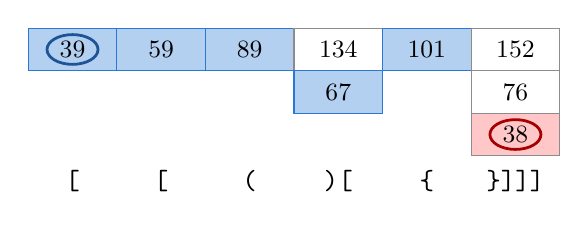
\begin{tikzpicture}[scale=0.9]\dropgridXXXIX
    \draw[black!45, fill=red!22] (6.25,-1.20) rectangle ++(1.25,-0.60);
    \node at (6.875,-1.500) {\small $38$};
    \draw[chordblue!70!black, line width=1pt] (0.625,-0.300) ellipse (0.36 and 0.21);
    \draw[red!65!black, line width=1pt] (6.875,-1.500) ellipse (0.36 and 0.21);
  \end{tikzpicture}}

\begin{document}
\maketitle

\begin{center}\small
  \copyright\ 2026 Ruud H.G. van Tol and Mike Winkler. Licensed under \href{https://creativecommons.org/licenses/by/4.0/}{CC BY 4.0}.
\end{center}

\section{Only go all the way down if needed}
\label{sec:intro}

\termhere{stepT}Take a positive integer $x$. If it is even, halve it. If it is odd, triple it,
add $1$, and halve the (now even) result. In one formula, the \keyterm{stepT}{step $T$}:
\[
T(x) = \begin{cases} x/2, & x \text{ even},\\ (3x+1)/2, & x \text{ odd}, \end{cases}
\]
the reduced Collatz function, OEIS A014682\index{OEIS!A014682}~\cite{OEIS_A014682}.
Starting from $7$, repeated steps give
\[
7 \to 11 \to 17 \to 26 \to 13 \to 20 \to 10 \to 5 .
\]
The well-known question is whether every start eventually reaches $1$. \termhere{drop}We ask
something smaller: does every $x > 1$ eventually fall \emph{below itself}? For
$7$ that happens after $7$ steps, at $5$. We stop right there, at the
\keyterm{drop}{drop}. In this paper we use the convention that $\mathrm{drop}(1) = 1$,
with trajectory $(1, 2, 1)$. For every $x > 1$, reaching $1$ is already a drop.
The two questions are equivalent: if every number drops, then every number
reaches $1$, because each drop lands on a smaller number, which drops in turn
(Lean: \lean{tDrop\_equiv\_collatzT} for $T$; \lean{drop\_equiv\_collatz} for the fast
map $R$ of Chapter~\ref{sec:fast}; \lean{rDrop\_iff\_tDrop} carries the drop question
from one to the other). From here on we only ever look at the way
to the drop, never beyond it.

\subsection*{Families that drop together}

\termhere{family}Take the odd numbers of the form $4i+1$: $1, 5, 9, 13, \dots$. One step gives
\[
\frac{3(4i+1)+1}{2} = \frac{12i+4}{2} = 6i+2,
\]
which is even, so the next step halves it to $3i+1$. (The number of factors $2$ in $6i+2$ is
A375961\index{OEIS!A375961}$(i)$~\cite{OEIS_A375961}.) So after two steps,
every number $4i+1$ has become $3i+1$, which is smaller as soon as $i \ge 1$.
(Whether $3i+1$ is odd or even depends on $i$; we don't need to know, because
we have already dropped.) The whole \keyterm{family}{family} $1, 5, 9, 13, \dots$ drops in two
steps: for $i = 0$ the two steps are $1 \to 2 \to 1$, the drop of $1$ by our
convention. We write this as
\[
1 + i\cdot 2^2 \;\to\; 1 + i\cdot 3^1 .
\]
The family $16i+3$ takes four steps:
$16i+3 \to 24i+5 \to 36i+8 \to 18i+4 \to 9i+2$, that is,
\[
3 + i\cdot 2^4 \;\to\; 2 + i\cdot 3^2 .
\]

% a page may end here: the next paragraph stays with Table 1
\pagebreak[0]
\termhere{p3}\termhere{p2}The mechanism is visible in the $i$-part. A halving divides it by $2$; an odd
step multiplies it by $3/2$. After \keysym{p2}{$p_2$} steps, \keysym{p3}{$p_3$} of them odd, the $i$-part
$i\cdot 2^{p_2}$ has become $i\cdot 3^{p_3}$. As long as there are enough
factors $2$ left in the $i$-part, it doesn't influence whether a number is odd
or even: every member of the family takes the same steps as its smallest
member. Here are the first families, sorted by $p_3$ (Table~\ref{tab:families}).

\nopagebreak
\begin{herefloat}{table}
$\begin{array}{r@{\;+\;i\cdot}l@{\quad\to\quad}r@{\;+\;i\cdot}l@{\qquad}l}
\toprule
\multicolumn{2}{c}{\text{family}} & \multicolumn{2}{c}{\text{after the drop}} & \quad\text{steps} \\
\midrule
1 & 2^2 & 1 & 3^1 & \bw{10} \\
3 & 2^4 & 2 & 3^2 & \bw{1100} \\
11 & 2^5 & 10 & 3^3 & \bw{11010} \\
23 & 2^5 & 20 & 3^3 & \bw{11100} \\
7 & 2^7 & 5 & 3^4 & \bw{1110100} \\
15 & 2^7 & 10 & 3^4 & \bw{1111000} \\
59 & 2^7 & 38 & 3^4 & \bw{1101100} \\
\bottomrule
\end{array}$
\caption{The first families: class id (Chapter~\ref{sec:numbers}) plus multiples of $2^{p_2}$, the values after the drop, and the steps.}
\label{tab:families}
\end{herefloat}

\termhere{steppattern}In the last column, \bw{1} is an odd step and \bw{0} a halving. Every family drops,
because $3^{p_3} < 2^{p_2}$ and the constant part drops too. And in this table the number of
steps is the same for a given $p_3$: it is the number of binary digits
of $3^{p_3}$. (That it is so for every family is the width identity of
Chapter~\ref{sec:open}.) For example, $3^4 = 81 = \bin{1010001}$ has $7$ digits.

\nopagebreak
Which \keyterm{steppattern}{step patterns} are possible, and how many are there for each $p_3$?
Chapter~\ref{sec:words} answers the first question exactly; the counts
from $p_3 = 1$ on, $1, 1, 2, 3, 7, 12, 30, 85, \dots$, form OEIS A100982\index{OEIS!A100982}~\cite{OEIS_A100982}.
With this the question becomes: \emph{does every $x > 1$ belong to some
family?} That is still open, and Chapter~\ref{sec:open} splits it into two
precise parts. What this paper shows is how the families are built, how to
count them, and how they sort:
% this list stays on one page, with the line before it
{\samepage
\begin{itemize}
\item A member of a family drops at the end of its pattern exactly when it lies above a
  single rational number, its \emph{cycle point} (Chapter~\ref{sec:numbers}).
\item Every step pattern splits at its record lows into smaller patterns, and
  whether pieces fit together depends only on their $p_3$
  (Chapter~\ref{sec:chain}).
\item The words are counted in three ways, one of them extended by M.~Winkler
  (A100982\index{OEIS!A100982}, Chapter~\ref{sec:count}).
\item Families, their step patterns, and the patterns of a faster map
  sort in the same order (Chapter~\ref{sec:fast}).
\end{itemize}}

\ifpaper\clearpage\fi
\subsection*{How this paper relates to Paper 1}

Paper~1~\cite{Paper1} tells the same story as a game, without proofs. This paper
gives the proofs, in the words of the literature and of the Lean formalization:
Paper~1's valid words are the admissible words here, its height is the level, its
Collatz-primes are the class ids, and its parts are the blocks. Every result cited with a Lean name is
proved in Lean~4 with Mathlib (open statements enter as hypotheses); Lean names are set in sans-serif, like
\lean{admissible\_iff\_chain} (namespace \lean{AcceleratedCollatz}). Examples use
the script \texttt{pv.py} of Paper~1, Appendix~\ref{P1-app:pv}.

Paper~1 reads its words off the real rides and stays shallow on purpose. What it
leaves out is here:
% this list stays on one page, with the word box
{\samepage
\begin{itemize}
\item the words defined by levels instead of rides, and every rule of Paper~1 proved
  for them (Chapter~\ref{sec:words}); whether levels and rides always agree is the
  width identity, and together with covering it is the open part
  (Chapter~\ref{sec:open});
\item the drop formula and the cycle point (Chapter~\ref{sec:numbers});
\item the exact gluing rule, the block factor and its records, brackets and other ways
  to cut (Chapter~\ref{sec:chain});
\item the counting formulas, first passages, active words and Winkler's bounds
  (Chapter~\ref{sec:count});
\item marked vectors and the sorting proofs (Chapter~\ref{sec:fast});
\item the finite check of the width identity up to Order $10\,781\,273$, and five side
  results (Chapter~\ref{sec:open}).
\end{itemize}}

\subsection*{Contributions}

M.~Winkler pointed to the classical ladder factorization behind the cuts, gave the
range form of the binomial identity and the deficit form of the budget, and asked the
question that led to the sweeps for every odd $q$.

\nopagebreak

\begin{wordbox}
\boxhere{stepT}step $T$\index{step T@\termlink{stepT}{step $T$}|textbf} & $x \mapsto x/2$ for even $x$, $x \mapsto (3x+1)/2$ for odd $x$. \\
\boxhere{drop}drop\index{drop@\termlink{drop}{drop}|textbf} & the first value below the start, and the step where it is reached. \\
\boxhere{family}family\index{family@\termlink{family}{family}|textbf} & all $x = c + i\cdot 2^{p_2}$ that take the same steps up to their
  drop; later called a \emph{class}, with \emph{class id} $c$. \\
\boxhere{p3}$p_3$ (Order)\index{p3@\termlink{p3}{$p_3$ (Order)}|textbf} & the number of odd steps up to the drop. \\
\boxhere{p2}$p_2$\index{p2@\termlink{p2}{$p_2$}|textbf} & the number of binary digits of $3^{p_3}$: the length of the word
  (Chapter~\ref{sec:words}) and, under the width identity, the number of steps up to the drop (Chapter~\ref{sec:open}). \\
\boxhere{steppattern}step pattern\index{step pattern@\termlink{steppattern}{step pattern}|textbf} & the odd steps (\bw{1}) and halvings (\bw{0}) up to the drop; later
  called an \emph{admissible word}. \\
A014682\index{OEIS!A014682} & the step $T$ in the OEIS. \\
A375961\index{OEIS!A375961} & factors $2$ in $6i+2$.
\end{wordbox}

%% ======================================================================
\section{Words and levels}
\label{sec:words}

Chapter~\ref{sec:intro} showed that inside a family only the step pattern
matters. Let us study the patterns on their own, without numbers.

\termhere{word}A \keyterm{word}{word} is a finite string of \bw{1}s and \bw{0}s. \termhere{level}Read it from left to right
and keep a running product, the \keyterm{level}{level}: start at $1$, multiply by $3/2$
for every \bw{1} and by $1/2$ for every \bw{0}. This is what happens to the
$i$-part of a family (Chapter~\ref{sec:intro}), so the level tells how a
family's members grow and shrink, ignoring the small ``$+1$'' of each odd step.
After a word with $n$ ones and length $L$, the level is $3^n/2^L$.

Table~\ref{tab:levels} shows the word \bw{1110100}, the pattern of $7 + i\cdot 2^7$.

\begin{table}[htbp]
\centering
$\begin{array}{l*{7}{c}}
\toprule
\text{letter} & \bw{1} & \bw{1} & \bw{1} & \bw{0} & \bw{1} & \bw{0} & \bw{0} \\
\midrule
\text{level}  & \tfrac32 & \tfrac94 & \tfrac{27}{8} & \tfrac{27}{16} &
                \tfrac{81}{32} & \tfrac{81}{64} & \tfrac{81}{128} \\
\bottomrule
\end{array}$
\caption{The levels of the word \bw{1110100}, letter by letter.}
\label{tab:levels}
\end{table}

The level stays above $1$ until the very last letter, and then falls below $1$.
That is the shape asked of a pattern: its level must not fall below $1$ too early,
and it must do so at the end.

\medskip\noindent
\termhere{admissible}A word is \keyterm{admissible}{admissible} if its level is above $1$ after every proper,
nonempty beginning (prefix), and below $1$ after the whole word
(Lean: \lean{Admissible}). \termhere{order}Its \keyterm{order}{Order} is its number of \bw{1}s.
\termhere{firstpassage}Admissible words are \keyterm{firstpassage}{first passages}: the first moment the level goes
below $1$.

\nopagebreak
\medskip
Three facts follow directly, and together they explain
Table~\ref{tab:families}.
\begin{itemize}
\item \emph{An admissible word ends with \bw{0}} (\lean{admissible\_last\_false}).
  A final \bw{1} would raise the level from at least $1$ to at least $3/2$.
\item \termhere{p2n}\emph{An admissible word of Order $n$ has length \keysym{p2n}{$p_2(n)$}, the number of
  binary digits of $3^n$} (\lean{admissible\_length}). Just before the final
  \bw{0} the level $3^n/2^{L-1}$ is at least $1$, and after it $3^n/2^L$ is below
  $1$, so $2^{L-1} \le 3^n < 2^L$. Equality holds only for the word \bw{0}: a power
  of $2$ is never a power of $3$, except $1 = 1$. These lengths are
  $1, 2, 4, 5, 7, 8, 10, \dots$ (A020914\index{OEIS!A020914}~\cite{OEIS_A020914}); from one Order to the next they grow
  by $1$ or $2$ (A022921\index{OEIS!A022921}~\cite{OEIS_A022921}).
\item \emph{No admissible word is a proper prefix of another}
  (\lean{admissible\_not\_prefix}). The shorter one already brings the level
  below $1$, which the longer one forbids.
\end{itemize}
The second fact says that the order of the letters doesn't change the length:
all admissible words of Order $n$ are rearrangements of $n$ ones and
$p_2(n) - n$ zeros. Here are all seven of Order $5$:
\[
\bw{11011010},\; \bw{11011100},\; \bw{11101010},\; \bw{11101100},\; \bw{11110010},\; \bw{11110100},\; \bw{11111000} .
\]
\termhere{lex}\termhere{rank}They are listed in \keyterm{lex}{lexicographic} (dictionary) order, which is also the order
in which \texttt{pv.py} numbers them: this is their \keyterm{rank}{rank}.

\termhere{oddpart}The \bw{0}s at the end of an admissible word carry no information: the Order
fixes the length. Read as a binary number, the word without them is the \keyterm{oddpart}{odd part}
of the word, its number divided by $2$ as often as possible
(A000265\index{OEIS!A000265}~\cite{OEIS_A000265}; \lean{encode\_core}, Lean: \lean{core}). For Order at
least $1$ it ends with the last \bw{1}, and filled up with \bw{0}s to the length $p_2$ it
gives the word back (\lean{keyPV\_core}, \lean{core\_keyPV}). So distinct admissible words, of any
Orders, have distinct odd parts (\lean{oddPart\_injective}). \texttt{pv.py} takes and prints
odd parts (\pv{list 5} begins with \texttt{1101101}) and computes all it prints from them;
\lean{attrs} does so in Lean.

\subsection*{Counting without listing}

The level after a prefix depends only on how many \bw{1}s and \bw{0}s it has, not on
their order. So a prefix is a point $(j,k)$ in a grid, $j$ ones and $k$ zeros,
and an admissible word is a walk from $(0,0)$ that, after its first step, stays in the region
$3^j > 2^{j+k}$ until its last step leaves it. \termhere{an}Counting walks is quick: add up
the counts of the two predecessors of each point. This gives
the number \keysym{an}{$a(n)$} of admissible words of Order $n$ (A100982\index{OEIS!A100982}, $n \ge 1$) without listing a single word; \pv{count 60} prints $a(60)$,
a $25$-digit number, instantly. The counts per grid point form the triangle
A368514\index{OEIS!A368514}~\cite{OEIS_A368514}, similar to the Catalan triangle but with $p_2(n) - n$
entries in row $n$; the last nonzero entry of its row $n+1$ is $a(n)$.

\nopagebreak
The same walk, counted by length instead of Order, gives two more sequences.
\termhere{active}A word whose level stays above $1$ all the way is \keyterm{active}{active}; there are
$1, 1, 1, 2, 3, 4, 8, 13, 19, \dots$ of length $k = 0, 1, 2, \dots$
(A076227\index{OEIS!A076227}~\cite{OEIS_A076227}). An active word followed by \bw{1} is active again;
followed by \bw{0} it is either active or admissible. So the admissible words of
length $k$ number $2\,\mathrm{A076227}\index{OEIS!A076227}(k-1) - \mathrm{A076227}\index{OEIS!A076227}(k)$; that count is nonzero only at
the lengths $k = p_2(n)$, where it equals $a(n)$ (for $n \ge 1$, and as far as the
width identity of Chapter~\ref{sec:open} holds, this is
A260591\index{OEIS!A260591}~\cite{OEIS_A260591}, which counts by dropping time).
So $a(n) = 2\,\mathrm{A076227}\index{OEIS!A076227}(p_2(n)-1) - \mathrm{A076227}\index{OEIS!A076227}(p_2(n))$ (\lean{card\_active\_succ},
\lean{card\_admSet\_add\_active}).

\subsection*{The word at a given rank}

The grid also gives the word at any rank without listing the others, as the
ballot numbers do for Dyck paths. Fix the Order $n$ and count backwards: let
$t(j,k)$ be the number of admissible words of Order $n$ that begin with a given
prefix at the point $(j,k)$. It is $1$ at the end point $(n,\, p_2(n) - n)$, and
inside the region
\[
t(j,k) = t(j,k+1) + t(j+1,k),
\]
where a term counts as $0$ if its point has more than $n$ ones, or lies outside
the region and is not the end point. Then $a(n) = t(1,0)$. Table~\ref{tab:tjk}
shows $t$ for $n = 5$, with the end point at $(5,3)$.

\begin{table}[htbp]
\centering
$\begin{array}{r ccccc}
\toprule
k \backslash j & 1 & 2 & 3 & 4 & 5 \\
\midrule
0 & 7 & 7 & 5 & 3 & 1 \\
1 & \cdot & 2 & 2 & 2 & 1 \\
2 & \cdot & \cdot & \cdot & 1 & 1 \\
3 & \cdot & \cdot & \cdot & \cdot & 1 \\
\bottomrule
\end{array}$
\caption{The backward count $t(j,k)$ for Order $5$: $j$ ones across, $k$ zeros down.}
\label{tab:tjk}
\end{table}

To write the word of rank $r$, start with \bw{1} at $(1,0)$. At the point $(j,k)$
let $z = t(j, k+1)$, the number of words that go on with \bw{0}. If
$r \le z$, write \bw{0}; otherwise write \bw{1} and replace $r$ by $r - z$. For
$n = 5$ and $r = 4$ the values of $z$ are $0, 2, 2, 0, 1, 1, 1$ and the word is
\bw{11101100} (\pv{unrank 5 4}). The other way, the rank of a word is $1$ plus
the sum of $z$ over its \bw{1}s after the first (\pv{rank}).

The table has no more than $n\,p_2(n)$ entries, and a word takes $p_2(n)$ steps.
For Order $60$, with $a(60) = 1325438036712274130536314$, the word of rank
$\lfloor 2\,a(60)/3 \rfloor = 883625357808182753690876$ is
\[
\begin{array}{l}
\bw{111111010001111111110110101001110101111011011011} \\
\bw{001011101011000101111101101011111100001100010100}
\end{array}
\]
with the class id $56358534677734342530833494207$. At Order $2000$, where $a(2000)$
has $902$ digits, this still takes less than a second. The table, the walk and
its inverse are also in Lean, with ranks counted from $0$: the table gives $a(n)$
(\lean{card\_admSet\_eq\_count}), and the walk and its inverse compute the sorted
enumeration of the words of an Order and its inverse (\lean{admIndex\_eq\_unrank},
\lean{admIndex\_symm\_eq\_rank}).

\subsection*{A warning about names}

Terras~\cite{Terras1976} used \emph{admissible} for a weaker condition: level
above $1$ after every proper prefix, with no condition at the end. In his words,
our admissible words are \emph{terminal}, and words whose level also stays
above $1$ at the end are \emph{active}. We follow the usage of OEIS A100982\index{OEIS!A100982}.
The two meet in one number: $a(n)$ is the entry of Terras's table for length
$p_2(n)$ with $p_2(n) - n$ zeros, since no word of that length and Order is
active.

\begin{wordbox}
\boxhere{word}word\index{word@\termlink{word}{word}|textbf} & a string of \bw{1}s (odd steps) and \bw{0}s (halvings). \\
\boxhere{level}level\index{level@\termlink{level}{level}|textbf} & the running product: $\times\frac32$ per \bw{1}, $\times\frac12$ per \bw{0};
  after the whole word it is $3^n/2^L$. \\
\boxhere{admissible}admissible word\index{admissible word@\termlink{admissible}{admissible word}|textbf} & level above $1$ after every proper nonempty prefix, below
  $1$ at the end; a first passage. Terras: \emph{terminal}. \\
\boxhere{firstpassage}first passage\index{first passage@\termlink{firstpassage}{first passage}|textbf} & the first prefix whose level is below $1$. \\
\boxhere{order}Order\index{order@\termlink{order}{Order}|textbf} & the number of \bw{1}s in a word. \\
\boxhere{p2n}$p_2(n)$\index{p2(n)@\termlink{p2n}{$p_2(n)$}|textbf} & the length of every admissible word of Order $n$: the number of
  binary digits of $3^n$. \\
\boxhere{an}$a(n)$\index{a(n)@\termlink{an}{$a(n)$}|textbf} & the number of admissible words of Order $n$ (A100982). \\
\boxhere{lex}lexicographic order\index{lexicographic order@\termlink{lex}{lexicographic order}|textbf} & dictionary order on words of equal length. \\
\boxhere{rank}rank\index{rank@\termlink{rank}{rank}|textbf} & position of a word in the lexicographic list of its Order. \\
\boxhere{oddpart}odd part\index{odd part@\termlink{oddpart}{odd part}|textbf} & a word without the \bw{0}s at its end; as a binary number, its odd
  part (A000265\index{OEIS!A000265}). \\
\boxhere{active}active word\index{active word@\termlink{active}{active word}|textbf} & level above $1$ after every nonempty prefix, including the
  whole word. \\
A368514\index{OEIS!A368514} & active prefixes counted by ones and zeros. \\
A020914, A022921\index{OEIS!A020914}\index{OEIS!A022921} & $p_2(n)$, and its increments $1$ or $2$. \\
A100982\index{OEIS!A100982} & $a(n)$, admissible words of Order $n$. \\
A076227, A260591\index{OEIS!A076227}\index{OEIS!A260591} & active, admissible words of length $k$ (A260591 as far as the width identity holds).
\end{wordbox}

%% ======================================================================
\section{From words to numbers: the cycle point}
\label{sec:numbers}

Now bring the numbers back. \termhere{parityword}The \keyterm{parityword}{parity word} of $x$ of length $L$ records
its first $L$ steps: \bw{1} for an odd step, \bw{0} for a halving.

\subsection*{Every word is a class}

\termhere{class}Which numbers have a given parity word $w$ of length $L$? Chapter~\ref{sec:intro}
already showed the mechanism: the first step is decided by the last binary
digit of $x$, the second step by the last two digits, and so on. Each step
fixes one more binary digit. \termhere{classid}So the numbers with parity word $w$ form exactly
one residue \keyterm{class}{class} modulo $2^L$:
\[
x = c + i\cdot 2^L, \qquad i = 0, 1, 2, \dots,
\]
where $1 \le c \le 2^L$ is its smallest positive member, the \keyterm{classid}{class id}
(Lean: \lean{tBits\_classId}, \lean{tBits\_congr}, \lean{modEq\_of\_tBits\_eq}; for
the admissible words of one Order, \lean{classEquiv}, \lean{classId\_tBits}). \termhere{collatzprime}For
admissible words we call
the class ids \keyterm{collatzprime}{Collatz-primes}. Grouped by Order, they are the rows of
A177789\index{OEIS!A177789}~\cite{OEIS_A177789}:
\[
2 \;\mid\; 1 \;\mid\; 3 \;\mid\; 11, 23 \;\mid\; 7, 15, 59 \;\mid\;
39, 79, 95, 123, 175, 199, 219 \;\mid\; \dots
\]
(A177789\index{OEIS!A177789} writes the Order-$0$ class as $0 \bmod 2$). Merged and sorted from
Order $2$ on, they form A243115\index{OEIS!A243115}~\cite{OEIS_A243115}:
$3, 7, 11, 15, 23, 27, 31, 39, 47, 59, \dots$. The smallest of each Order,
$2, 1, 3, 11, 7, 39, \dots$, is A122442\index{OEIS!A122442}~\cite{OEIS_A122442} (which has
$5$ in the place of the $1$: the smallest member above $1$). These three sequences are
defined by dropping times; they are our class ids as far as the width identity of
Chapter~\ref{sec:open} holds.

\subsection*{The drop formula}
\phantomsection\label{sec:dropformula}

\termhere{rho}Each odd step adds a $1$ before halving. Following these $+1$s through the
remaining steps shows that for every $x$ whose first $p_2$ steps follow an
admissible word $w$ of Order $p_3$,
\[
T^{p_2}(x) = \frac{3^{p_3}\,x + \rho}{2^{p_2}},
\]
where \keysym{rho}{$\rho$} is an integer that depends only on $w$, positive when the Order
is at least $1$ (Lean: \lean{rho}, \lean{rho\_pos\_iff}). For $w = \bw{11010}$, class id $11$: $\rho = 23$, and indeed
$(27\cdot 11 + 23)/32 = 320/32 = 10$. Replacing $x$ by $x + i\cdot 2^{p_2}$
adds exactly $i\cdot 3^{p_3}$ to the result: that is the family rule
$c + i\cdot 2^{p_2} \to d + i\cdot 3^{p_3}$ of Chapter~\ref{sec:intro}
(\lean{tStep\_iterate\_shift}; in terms of the drop, for a class id above its
cycle point, \lean{affine\_classId}).

\nopagebreak
Since the result is an integer, $3^{p_3}c + \rho$ is divisible by $2^{p_2}$. As $3$ is
invertible modulo $2^{p_2}$, this finds the class id directly:
\[
c \equiv -\rho \cdot 3^{-p_3} \pmod{2^{p_2}}.
\]
For \bw{11010}: $27^{-1} \equiv 19$ and $-23 \cdot 19 \equiv 11 \pmod{32}$. This is
how \texttt{pv.py} computes class ids.

\subsection*{Who drops: above the cycle point}

\termhere{d23}A member $x$ drops at the end exactly when $3^{p_3} x + \rho < 2^{p_2} x$, that
is, when
\[
\rho < d_{23}\, x, \qquad \keysym{d23}{d_{23}} = 2^{p_2} - 3^{p_3},
\]
(\lean{drop\_iff\_rho}). And no member drops \emph{before} the end, because
every proper prefix has level above $1$ (\lean{no\_drop\_before}). \termhere{cyclepoint}Write
$x^* = \rho / d_{23}$. Then:
\[
\text{\emph{a member of the class drops at the end of its word
if and only if it is larger than $x^*$.}}
\]
The number $x^*$ is the \keyterm{cyclepoint}{cycle point} of the word: an integer $x = x^*$
that plays the word would come back to itself
(\lean{fixed\_iff\_rho}). Table~\ref{tab:cycle} shows some examples.

\nopagebreak
\begin{herefloat}{table}
$\begin{array}{r l r r l}
\toprule
\text{class id} & \text{word} & \rho & d_{23} & x^* \\
\midrule
1 & \bw{10} & 1 & 1 & 1 \\
3 & \bw{1100} & 5 & 7 & 5/7 \\
11 & \bw{11010} & 23 & 5 & 23/5 \\
7 & \bw{1110100} & 73 & 47 & 73/47 \\
39 & \bw{11101100} & 251 & 13 & 251/13 \\
\bottomrule
\end{array}$
\caption{Cycle points $x^* = \rho/d_{23}$ of the first words.}
\label{tab:cycle}
\end{herefloat}

The first line explains why $1$ drops only onto itself: it \emph{is} its own
cycle point, with trajectory $(1, 2, 1)$. Every other member of that class,
$5, 9, 13, \dots$, lies above it and drops.

The cycle point carries more. Its denominator $d_{23}$ is odd and not divisible by
$3$, so $x^*$ can be read modulo powers of $2$ and of $3$. Read modulo $2^{p_2}$,
it \emph{is} the class id; read modulo $3^{p_3}$, it is $T^{p_2}$ of the class id (its drop, if it drops there). For
$x^* = 23/5$: $23 \cdot 5^{-1} \equiv 11 \pmod{32}$ and
$23 \cdot 5^{-1} \equiv 10 \pmod{27}$. One rational number, three readings:
its $2$-adic digits give the start, its $3$-adic digits the drop, and its size
decides whether the drop happens.

\termhere{q}How close does a class id come to its cycle point? The ratio $\keysym{q}{q} = x^*/x$ must
be below $1$ for the class id to drop. Among all admissible words of
Orders $2$ to $15$ the largest ratio is $q = 251/507$, at $x = 39$
(\pv{maxq 2 \dots\ 15}). Among the class ids below $20\,000\,000$ the tightest case is $x = 47$ (Order $34$), whose
cycle point lies between $33$ and $34$. For $27$, whose way to the
drop takes $59$ steps, the cycle point lies between $8$ and $9$: far below.
Whether \emph{every} class id above $1$ lies above its cycle point is open; it is the
width identity of Chapter~\ref{sec:open}, checked there for every Order up to
$10\,781\,273$.

\nopagebreak
All residues modulo $2^k$ together, with the step $T$, form a De Bruijn graph
(Laarhoven and de Weger~\cite{deWeger2012}); the admissible classes are a sparse,
special part of it.

\begin{wordbox}
\boxhere{parityword}parity word of $x$\index{parity word@\termlink{parityword}{parity word}|textbf} & its first $L$ steps: \bw{1} odd, \bw{0} halving. \\
\boxhere{class}class\index{class@\termlink{class}{class}|textbf} & all $x$ with the same parity word of length $L$; a residue class
  modulo $2^L$. \\
\boxhere{classid}class id\index{class id@\termlink{classid}{class id}|textbf} & the smallest positive member of a class. \\
\boxhere{collatzprime}Collatz-prime\index{collatz-prime@\termlink{collatzprime}{Collatz-prime}|textbf} & a class id of an admissible word. \\
A177789, A243115\index{OEIS!A177789}\index{OEIS!A243115} & class ids by Order; all of Order $\ge 2$, sorted (as far as the width identity holds). \\
A122442\index{OEIS!A122442} & the smallest class id of each Order (as far as the width identity holds). \\
\boxhere{rho}$\rho$\index{rho@\termlink{rho}{$\rho$}|textbf} & the integer with $T^{p_2}(x) = (3^{p_3}x + \rho)/2^{p_2}$. \\
\boxhere{d23}$d_{23}$\index{d23@\termlink{d23}{$d_{23}$}|textbf} & $2^{p_2} - 3^{p_3}$, positive for admissible words. \\
\boxhere{cyclepoint}cycle point $x^*$\index{cycle point@\termlink{cyclepoint}{cycle point $x^*$}|textbf} & $\rho/d_{23}$; members above it drop at the end,
  none drop earlier. \\
\boxhere{q}$q$\index{q@\termlink{q}{$q$}|textbf} & $x^*/x$; the class id drops when $q < 1$.
\end{wordbox}

%% ======================================================================
\section{The chain decomposition}
\label{sec:chain}

This chapter is the heart of the paper: a way to cut any admissible word into
smaller admissible words, and to glue them back.

\subsection*{Cutting at record lows}

\termhere{recordlow}Take an admissible word of Order at least $1$. It starts with \bw{1}, so the level
begins at $3/2$. Now cut the rest each time the level reaches a new \keyterm{recordlow}{record
low}, that is, each time the piece since the last cut first brings its own
product below $1$. For the word \bw{11011010} (class id $123$):
\[
\bw{1} \;\big|\; \bw{10} \;\big|\; \bw{11010},
\qquad
\text{levels at the cuts: } \tfrac32 \;\to\; \tfrac98 \;\to\; \tfrac{243}{256}.
\]
\termhere{block}Each piece is an admissible word in its own right: \bw{10} has Order $1$ and
\bw{11010} has Order $3$. We call such pieces \keyterm{block}{blocks}. The cut positions
are exactly the moments where the level is lower than ever before, counted from the
leading \bw{1} on
(\lean{isRecordLow\_iff\_cut}, \lean{exists\_chain\_recordLow}). Cutting a
path at these \emph{descending ladder epochs} is a classical
idea~\cite{Feller1971}, as M.~Winkler pointed out; what is new here is what it gives for admissible words:
the condition below, which depends on the Orders only, and the counts of
Chapter~\ref{sec:count}.

\begin{theorem}[Chain decomposition]
\label{thm:chain}
\termhere{chain}Every admissible word of Order $n+1$ is, in exactly one way, a \keyterm{chain}{chain}
\[
1 \; A_1 A_2 \cdots A_k \; t,
\]
\termhere{tail}with $k \ge 0$ admissible blocks $A_1, \dots, A_k$ of Orders $o_1, \dots, o_k \ge 1$,
$o_1 + \dots + o_k = n$, and a \keyterm{tail}{tail} $t$ that is empty or a single \bw{0}.
Conversely, admissible blocks of any such Orders glue together in this way into an
admissible word if and only if the level at the cut before the last block is above $1$:
\[
2^{\,1 + p_2(o_1) + \dots + p_2(o_{k-1})} \;<\; 3^{\,1 + o_1 + \dots + o_{k-1}},
\]
and then the tail is forced: it is \bw{0} exactly when the inequality also holds
with $o_k$ included.
\end{theorem}
Lean: \lean{exists\_chain}, \lean{chain\_unique}, \lean{admissible\_iff\_chain},
\lean{validOrders\_iff\_dropLast}; the tail in terms of $p_2$, \lean{tail\_eq\_zero\_iff}.

\medskip
\emph{Why it works.} Cutting at the record lows gives the blocks: each piece is the
shortest one with product below $1$, so it is admissible, and a last piece \bw{0} is
the tail. Inside a block, the level is the level at the block's start
times a prefix product of the block, and both are above $1$. So the only places
where the level can fail are the block boundaries, and there the level is
$3^{1+o_1+\dots+o_i}/2^{1+p_2(o_1)+\dots+p_2(o_i)}$, which depends only on the
Orders. Each block lowers the level, so it suffices to check the last inner
cut. Uniqueness comes from the prefix fact of Chapter~\ref{sec:words}.

\nopagebreak
The surprise is the second half: \emph{which} blocks are used doesn't matter at
all, only their Orders. The seven words of Order $5$ show it (\pv{list 5}, Table~\ref{tab:order5}).

\begin{table}[htbp]
\centering
$\begin{array}{r l l}
\toprule
\text{class id} & \text{word} & \text{chain} \\
\midrule
123 & \bw{11011010} & \bw{1}\,|\,\bw{10}\,|\,\bw{11010} \\
219 & \bw{11011100} & \bw{1}\,|\,\bw{10}\,|\,\bw{11100} \\
199 & \bw{11101010} & \bw{1}\,|\,\bw{11010}\,|\,\bw{10} \\
39  & \bw{11101100} & \bw{1}\,|\,\bw{1101100} \\
79  & \bw{11110010} & \bw{1}\,|\,\bw{11100}\,|\,\bw{10} \\
175 & \bw{11110100} & \bw{1}\,|\,\bw{1110100} \\
95  & \bw{11111000} & \bw{1}\,|\,\bw{1111000} \\
\bottomrule
\end{array}$
\caption{The seven admissible words of Order $5$ and their chains.}
\label{tab:order5}
\end{table}

The Orders $(1,3)$, $(3,1)$ and $(4)$ appear, each with every choice of blocks:
$1\cdot 2$, $2 \cdot 1$ and $3$ words. The other five, such as $(2,2)$ or $(1,1,2)$,
never appear: they pass level $1$ too early.

\subsection*{Chains as codes}

\termhere{validorders}Theorem~\ref{thm:chain} gives a bijection: on one side the admissible words of Order
$n+1$, on the other the lists of blocks with \keyterm{validorders}{valid Orders} (Orders that satisfy its
inequality) that add up to $n$
(\lean{chainEquiv}). \termhere{code}A block is an admissible word itself, known by its Order and
its rank (Chapter~\ref{sec:words}). A word can be written as a short list of
pairs (Order, rank), one per block: its \keyterm{code}{code}. The leading \bw{1} is not
listed, and the tail follows from the Orders. This is a bijection as well
(\lean{codeEquiv}). For \bw{11011010} the blocks \bw{10} and \bw{11010} are the
first words of Orders $1$ and $3$, so its code is $(1,1), (3,1)$; \bw{11101100}
has the single block \bw{1101100}, the first word of Order $4$, and the code
$(4,1)$. Both maps are computed by one pass that takes, again and again, the
shortest piece with product below $1$ (\lean{chainEquiv\_eq\_chainOf},
\lean{codeEquiv\_eq\_codeOf}). In Lean the ranks count from $0$;
\texttt{pv.py} counts from $1$ and lists a tail as $(0,1)$ (\pv{attrs 11}, for \bw{1100}).

The odd part of a word answers a what-if. Stop an odd start $x > 1$ that drops at the end of its
admissible word, not at its drop but as soon as the odd part of the value is below $x$. From the last odd step on
only halvings remain, down to the drop value $d < x$; there the odd part of the
value is that of $d$, which is below $x$. Earlier it is not: a value $2^k m$
with $m$ odd and below $x$ would halve straight down to $m$, with no odd step
left. This stop comes right after the last odd step: its word is the odd part, and
the odd part of its value is that of the drop value. Classes, Orders and counts stay as
they are. But the odd parts of one Order differ in length, and one can begin
another (\bw{1} begins \bw{11}), so the three facts of
Chapter~\ref{sec:words} are lost. We keep the drop.

\subsection*{The block factor}

\termhere{blockfactor}A block of Order $o$ multiplies the level by its \keyterm{blockfactor}{block factor}
$f(o) = 3^{o}/2^{p_2(o)}$, which
lies between $1/2$ and $1$: for example $f(1) = 3/4$, $f(3) = 27/32$ and
$f(5) = 243/256$. Starting from $3/2$, the level must stay above $1$ at the last
inner cut. This is a \emph{budget}: the product of the block factors of all blocks
but the last must stay above $2/3$. For the chain $\bw{1}\,|\,\bw{10}\,|\,\bw{11010}$ it is
$f(1) = 3/4 > 2/3$ (Figure~\ref{fig:budget}). M.~Winkler phrased the same budget with logarithms: the
deficits $1 - \{o \log_2 3\}$ of those blocks must add up to less than
$\log_2 3 - 1$. So long chains need blocks with $f(o)$ close to $1$. The Orders where
$f(o)$ sets a new record are
\[
1,\ 3,\ 5,\ 17,\ 29,\ 41,\ 94,\ 147,\ 200,\ 253,\ 306,\ \dots
\]
(Figure~\ref{fig:blockfactor}; \pv{records 306}).
These are the denominators of the upper convergents and semiconvergents of
$\log_2 3$ (\lean{upperRecord\_iff\_semiconv}): the fractions on the Stern--Brocot path towards a number are its simplest
upper and lower approximations, and the runs of the path are the quotients of Euclid's
algorithm~\cite[\S4.5, pp.~122--123]{GKP1989}; M.~Winkler~\cite{Winkler2026b} links them
to the admissible words. Together with the lower ones (\lean{lowerRecord\_iff\_semiconv}) they
form A206788\index{OEIS!A206788}~\cite{OEIS_A206788}. Walking down the Stern--Brocot tree of
fractions towards $\log_2 3$ (K.~Ryde~\cite{Ryde2020}), these record Orders are
exactly the denominators of the fractions on the walk that lie above
$\log_2 3$ (\lean{upperRecord\_iff\_sbWalk}). In terms of $p_2$ alone: $p_2(a + b)$ is
$p_2(a) + p_2(b)$ or one less. At
a record Order $n$ it is one less for every split $n = a + b$ into positive parts
(\lean{upperRecord\_iff\_add}). At the Orders where $f$ comes closer to $1/2$ than ever
before, the \emph{lower} record Orders $1, 2, 7, 12, 53, \dots$, it is the full sum for
every split (\lean{lowerRecord\_iff\_add}), and they are the denominators of the fractions
below $\log_2 3$ on that walk (\lean{lowerRecord\_iff\_sbWalk}); the record Orders above are the
\emph{upper} ones. The first word of each Order (rank $1$) takes every halving that
keeps the level above $1$ (\lean{unrank\_zero}). After $a$ of its odd steps and their
halvings (not the final one) its level is $2 f(a)$, and every other level before its end is
above $2$. So its chain is cut exactly there for the lower record Orders $a$ up to its
own Order (\lean{isRecordLow\_firstWord}): its blocks are the first words of the Orders
$1, 5, 5, 41, 306, 306, \dots$, the gaps between neighbouring lower record Orders, and
of the rest (\lean{firstWord\_chain}; \pv{first 53}). Each such gap is an upper record Order
(\lean{upperRecord\_sub\_of\_lowerRecord}). Taken again for the rest, the first word of
Order $n$ is the first words of $a_1, a_2, \dots$, each without its final halving, then one
halving, where $a_1$ is the largest lower record Order up to $n$, $a_2$ the largest up to
$n - a_1$, and so on (for $n = 30$: $12, 12, 2, 2, 2$; \lean{firstWord\_eq\_greedy}).

\begin{figure}[htbp]
\centering
\begin{tikzpicture}\blockfactorplot\end{tikzpicture}
\caption{The block factor $f(o) = 3^o/2^{p_2(o)}$ for the Orders $1$ to $100$, on a
logarithmic scale between $1$ and $1/2$. Blue: the Orders where $f(o)$ comes closer
to $1$ than ever before, the record Orders of the text; orange: those where it comes
closer to $1/2$ ($1$ is both). Dashed: the budget $2/3$. A block above the dashed
line can stand first in a chain of two or more blocks; one below it can only be the
last block.}
\label{fig:blockfactor}
\end{figure}

\begin{figure}[htbp]
\centering
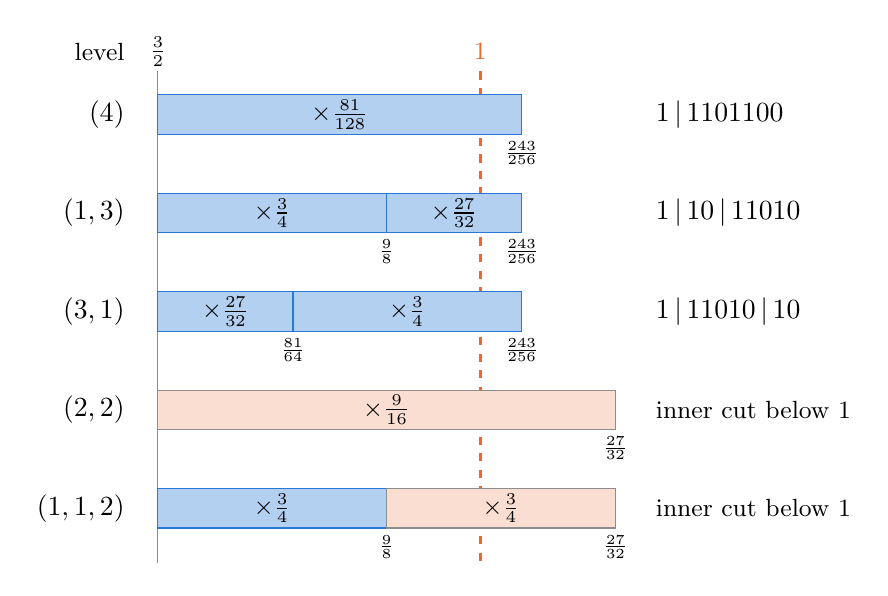
\begin{tikzpicture}\chainbudget\end{tikzpicture}
\caption{The budget of a chain, for Order $5$, with the level on a logarithmic
scale. Every chain starts at level $3/2$, after the leading \bw{1}, and each block
multiplies the level by its block factor; the level at each cut is written below
it. Every block but the last must end above level $1$ (dashed). The Orders $(4)$,
$(1, 3)$ and $(3, 1)$ fit, each shown with one of its words; all three end at
$243/256$, so their tail is empty. With $(2, 2)$ and $(1, 1, 2)$ an inner cut falls
below $1$.}
\label{fig:budget}
\end{figure}

\subsection*{Brackets}
\phantomsection\label{sec:brackets}


\termhere{bracketword}Open a bracket at every odd step of a word, and close it where the level first
falls below the level just before that odd step. For each odd step, count the
brackets that close before the next odd step; this list of counts is the
\keyterm{bracketword}{bracket word}. It is enough to rebuild the word: two admissible words with
the same bracket word are equal (\lean{bracketWord\_injective}). The reason is
short. For every level $\ell$ above $1$ and up to the current level, some open bracket
was opened at a level of at most $\ell$ and above $\ell/2$ (\lean{lvl\_gap}), so every halving closes at least
one bracket (\lean{closesAt\_pos\_of\_halving}); at the first place where two words
differ, the one with the halving closes more brackets before the next odd step. For
odd $q \ge 5$ (the sweeps below) an odd step opens $e$ brackets, $e$ the
largest with $2^e \le q$, at $1, 2, \dots, 2^{e-1}$ times that level; then too the word
is rebuilt (\lean{bracketWordQ\_injective}), with one bracket not (for $q = 5$: \bw{10100}, \bw{11000}).

On a trajectory brackets can be read off the values too: open at every odd
value, close at its first drop (Figure~\ref{fig:grid39}). A value cannot fall below its
bracket's start before the level does (\lean{exists\_lvlDrop\_le\_of\_isFirstDrop}). With
the width identity at the start of a bracket, both close at the same step
(\lean{lvlDrop\_iff\_isFirstDrop}):
under it for every start, every level close in an admissible word is the drop of the bracket's start, with
$\mathrm{drop}(1) = 1$ (\lean{lvlDrop\_iff\_isTDrop}). For $39$ both give the bracket line of
Figure~\ref{fig:grid39}; they agree for every odd start up to $200\,000$, at each of
the $596\,245$ floors on its way to the drop, in words of at most $135$ letters (an
exact computation outside Lean).

\begin{figure}[htbp]
\centering
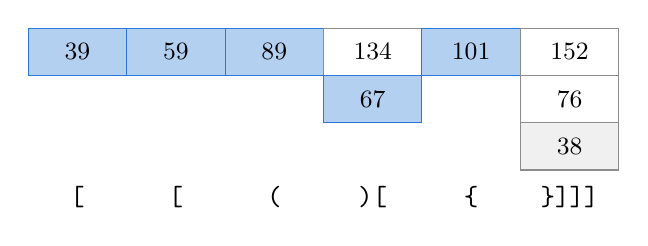
\begin{tikzpicture}\dropgridXXXIX\end{tikzpicture}
\caption{The drop grid of $39$: the start, then one column per odd step, with the value
it gives and the halvings after it below; odd values are shaded blue; $39$ drops to $38$ after $8$ steps. Under each column,
the brackets that open and close there. Every bracket opens at an odd value and
closes where the value first falls below it: with ) at an odd value, with \} at
an even value, with ] at the final drop.}
\label{fig:grid39}
\end{figure}

In the grid of Chapter~\ref{sec:words}, the walk of a word of Order $n \ge 1$ ends at
$(n, p_2(n) - n)$, which is $2n - p_2(n)$ steps short of the diagonal. \termhere{sharedclose}Every
bracket closes, and only after a halving, so the bracket word is a Dyck path with
$n$ up and $n$ down steps (\lean{sum\_bracketWord}, \lean{sum\_colCount\_lt\_le}).
The down steps are the halvings of the word and $2n - p_2(n)$ \keyterm{sharedclose}{shared closes}: where one
halving closes several brackets at once, every close after the first (\lean{halvings\_le\_colCount},
\lean{sum\_sharedCloses}).
Winkler's rational Dyck paths at the record Orders~\cite{Winkler2026b} use the
halvings alone; the bracket word adds where the shared closes fall.

Which Dyck paths are bracket words? Theorem~\ref{thm:chain} answers it. In the
chain $1\,A_1 \cdots A_k\,t$ every bracket of a block closes inside that block,
and the bracket of the leading \bw{1} closes at the very end. So the bracket word
of the chain is a $0$ followed by the bracket words of $A_1, \dots, A_k$, with $1$
added to the last entry (\lean{bracketWord\_chain}); the word \bw{10} has the
bracket word $(1)$. For example $\bw{1}\,|\,\bw{10}\,|\,\bw{11010}$ gives $0$, then
$(1)$ and $(0, 1, 2)$, and so $(0, 1, 0, 1, 3)$ (\pv{brackets 1101101}).
\termhere{brackettree}Read the Dyck path as a plane
tree, the \keyterm{brackettree}{bracket tree}: a node for every bracket, and as its children
the brackets opened directly inside it. Then the children of a node are the
blocks of the word its bracket spans. So a Dyck path with $n \ge 1$ up steps is the
bracket word of an admissible word of Order $n$ exactly when its tree has one
root and, at every node, the sizes of the children's subtrees are valid Orders
(\lean{image\_bracketWord\_admSet}). Only $p_2$ enters. A parser that reads the
list once decides it (\lean{isBracketTree\_iff}). The same
pass, keeping the words of the children instead of their sizes, decodes a bracket
tree back into its word (\lean{bracketDecode}, \lean{invOn\_bracketDecode}), so
the bracket trees with $n$ nodes number $a(n)$ (\lean{ncard\_isBracketTree}). Of the
$208012$ Dyck paths with $12$ up steps, $a(12) = 2652$ are bracket words.

\subsection*{Sweeps}
\phantomsection\label{sec:sweeps}
\termhere{ratcatalan}\termhere{sweepmap}The levels of a word are those of \keyterm{ratcatalan}{rational Catalan} combinatorics. Armstrong, Loehr and
Warrington~\cite{ALW2014} give the lattice point $(x, y)$ the level $by - ax$;
for coprime $a, b$ the levels along a path are distinct, as ours are because
$2^j \ne 3^o$. Their \keyterm{sweepmap}{sweep map}~\cite{ALW2015} sorts the steps of a path by level. As in
Thomas and Williams~\cite{ThomasWilliams2018}, each step sits at the level where it
ends, and steps are read from the highest level down. On admissible words the
final halving stays last (\pv{sweep 110111}). That the sweep of an admissible word is
admissible again is proved directly
(\lean{sweep\_mem\_admSet}): a prefix of the sweep collects the steps ending at or
above some level $\ell > 1$, each run of consecutive such steps climbs from below $\ell$
to at least $\ell$, so together they multiply to more than $1$. That no two words
sweep to the same one is the deep part. Integer weights with a ratio close enough to $\log_2 3$
order the lattice points of Order $n$ like our levels
(\lean{exists\_weights}, \lean{q\_pow\_lt\_iff\_weights}); with them an admissible word without its final halving is
a Dyck word in their sense (\lean{dropLast\_mem\_dyckSetQ}), and our sweep is theirs (\lean{sweep\_eq\_sweepZ}).
They proved that the sweep is a bijection on all words with given
numbers of both steps~\cite[Thm.~6.3]{ThomasWilliams2018}, so the sweep permutes the admissible
words of each Order (\lean{sweep\_bijOn}, with their theorem as hypothesis).

\termhere{startsweep}Sorting by the level at which each step \emph{starts}, lowest first, gives another
map, the \keyterm{startsweep}{start sweep}. On every word it is the sweep of the reversed word
(\lean{startSweepQ\_eq\_sweepQ\_reverse}); for all words, not only Dyck words,
so the start sweep is one-to-one on the admissible words of every Order
(\lean{startSweep\_injOn}, again with that theorem as hypothesis). It sends the admissible
words of Order $n$ to admissible words exactly at the upper record Orders $1, 3, 5, 17, 29, \dots$
(\lean{mapsTo\_startSweep\_iff}), and there it permutes them (\lean{startSweep\_bijOn\_iff}, same hypothesis).
At an upper record Order, a later point of an admissible word, except its end, that lies
below an earlier one has a level below $f(n)$ times the earlier level, $f(n)$ being the
level of the whole word (\lean{lvlQ\_lt\_mul\_of\_upperRecordQ}). So the word with its part
before the highest point reversed, and its part after it reversed, is admissible again, and
its sweep is the start sweep of the word (\lean{peakFlip\_mem\_admSetQ},
\lean{startSweepQ\_eq\_sweepQ\_of\_upperRecordQ}). At an Order $n$ that is not an upper
record, some split $n = a + b$ has $p_2(n) = p_2(a) + p_2(b)$. Take the word of $n$ odd
steps followed by halvings: its steps that start below the level $(3/2)^b$ come first in
its start sweep and multiply to $f(b) < 1$, so that start sweep is not admissible
(\lean{startSweepQ\_upDownQ\_not\_mem}).

\termhere{cutsweep}With the final halving left out and put back after the sorting, the \keyterm{cutsweep}{cut
sweep}, the result is admissible at every Order (\lean{cutSweep\_mem\_admSet}). A prefix of
the cut sweep holds the steps that start below some level $\ell > 1$; these multiply to at
least $\ell$ or to at least the level before the final halving, whichever is smaller
(\lean{min\_le\_prod\_of\_lower}). Both are above $1$, and the final halving still takes
the whole below $1$. The cut sweep permutes the admissible words exactly at the lower
record Orders $1, 2, 7, 12, 53, \dots$ (\lean{cutSweep\_bijOn\_iff}, with the same
hypothesis), by the same reversal around the highest point. At every other Order $n$ the
split $n = a + b$ with $f(a)$ least has $p_2(n) + 1 = p_2(a) + p_2(b)$; then the words of $a$ and of $b$ odd
steps followed by halvings, each without its final halving, and one halving after them,
form an admissible word (\lean{append\_cut\_mem\_admSetQ}) that passes a point lower than
the one before its final halving. Its steps up to that point cannot come first in any cut
sweep, so it is no cut sweep (\lean{not\_surjOn\_cutSweepQ}), and two words have the same
one (\lean{not\_injOn\_cutSweep}).

The record Orders are exactly the Orders at which the linear levels of
slope $p_2(n)/n$, or $(p_2(n) - 1)/n$ at the lower ones, order the lattice points
up to its end like ours, the two end points of the line apart: it puts those two at the same
level (\lean{gridLinear\_iff\_upperRecord},
\lean{gridLinear\_iff\_lowerRecord}; that these are exactly the record Orders of the block
factor, \lean{upperRecord\_iff\_blockFactor}, \lean{lowerRecord\_iff\_blockFactor}).
None of this needs the number $3$: the sweeps (same hypothesis) and the record Orders, also on
their walk (\lean{upperRecordQ\_iff\_sbWalkQ}), hold
for the words of every odd multiplier $q \ge 3$ (not the ratio $q$ of Chapter~\ref{sec:numbers}), with the factor $q/2$ for an odd step, the
admissible $qx+1$ sequences of Winkler~\cite{Winkler2026b}. \termhere{fillerzero}So is Theorem~\ref{thm:chain}, where for $q \ge 5$ blocks \bw{0}, the \keyterm{fillerzero}{filler zeros}, can
stand among the blocks, not only at the end (\lean{admissibleQ\_iff\_exists\_chainQ},
\lean{isRecordLowQ\_iff\_cut}), and so
is the first word of each Order as a chain of first words (\lean{firstWordQ\_chain},
\lean{firstWordQ\_blocks}). Neighbouring
upper record Orders differ by a lower one (\lean{lowerRecord\_sub\_of\_upperRecord}).

With the filler zeros as leaves and the odd steps as nodes, the words of every odd $q \ge 3$
are trees again: the admissible words of Order $n$ are the trees with $n$ nodes in which,
at every node, the Orders of the children keep the level above $1$ before the last child
and bring it below $1$ after it (\lean{word\_bijOn\_validTreesQ}). One pass reads the
tree off the word (\lean{parseTreeQ\_eq\_some\_iff}). One pass also reads it back from the
bracket word, with a count of the closes still due in the current column, filler zeros
included (\lean{decodeQ\_bracketWordQ}). With one bracket per odd step a filler zero adds
nothing to the counts (\lean{bracketWordOneQ\_chain}), which is why \bw{10100} and
\bw{11000} clash for $q = 5$, and two words of Order $2$ clash for every odd $q \ge 5$
(\lean{not\_injOn\_bracketWordOneQ}).

In terms of levels, a bracket closes at the first later point of lower level.
Scaled by $2^L$, the level of the point after $j$ steps with $o$ odd ones is the
integer $3^o\,2^{L-j}$, a $3$-smooth number (A003586\index{OEIS!A003586}~\cite{OEIS_A003586}).
The sweep sorts the points by their place among the $3$-smooth numbers, which
Mintz~\cite{Mintz1981} counted exactly: below $2^j 3^i$ there are
$ij + \sum_{k=1}^{i} p_2(k) + \sum_{k=1}^{j} u(k)$ of them, with $u(k)$ the number of
powers of $3$ below $2^k$ (\lean{card\_smoothBelowAt}; \pv{smooth 51} prints $2^5 3^4$).
Listed in increasing order, the $3$-smooth numbers walk through their grid by record
steps only (Figure~\ref{fig:smooth}). From $2^j 3^i$ the next one is $1/f(b)$ times it,
for the last upper record Order $b \le i$ ($b = 0$ is the doubling), or $2 f(a)$ times it,
for the last lower record Order $a \ge 1$ with $p_2(a) - 1 \le j$, if there is one: the smaller of the two
(\lean{smooth\_next}, \lean{smooth\_succ}, \lean{smooth\_succ\_of\_pow\_three}).
Those of $B \ge 2$ binary digits are $2^{B - p_2(i)}\,3^i$ for the Orders $i < u(B)$; with
$a$ and $b$ the last lower and upper record Orders below $u(B)$, they rise along
$i = ka \bmod (a+b)$, $k = 0, 1, \ldots$, skipping $i \ge u(B)$
(\lean{smooth\_digits}, \lean{exists\_mul\_mod\_eq\_of\_lastRecords},
\lean{smooth\_class\_mul\_mod\_lt}).

\begin{figure}[htbp]
\centering
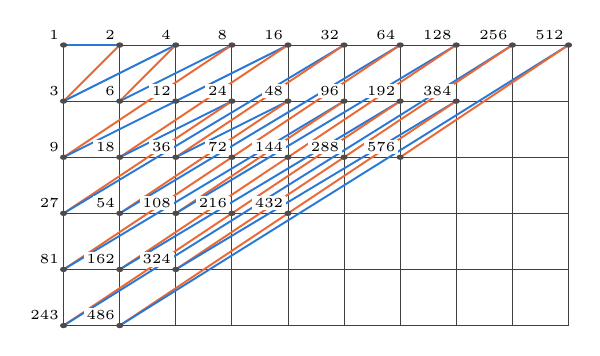
\begin{tikzpicture}[yscale=0.75]\smoothpath\end{tikzpicture}
\caption{The $3$-smooth numbers up to $576$ on the grid of Mintz~\cite{Mintz1981}, powers
of $2$ to the right and powers of $3$ downwards (his go up), joined in increasing order. Blue: the steps $1/f(b)$ for the upper record
Orders $b = 0, 1, 3, 5$. Orange: the steps $2 f(a)$ for the lower record Orders $a = 1, 2$.}
\label{fig:smooth}
\end{figure}

\subsection*{Other ways to cut}

Other recent work cuts the same words differently. Winkler~\cite{Winkler2026a}
cuts them at occurrences of the local pattern \bw{011} and counts them with a
run-composition recurrence; in~\cite{Winkler2026b} the blocks are runs, each
odd step with the halvings after it. Nakanishi~\cite{Nakanishi2026} and
Hikawa~\cite{Hikawa2026} remove the last \bw{1} (Chapter~\ref{sec:count}). These
cuts depend on local patterns; the cuts of Theorem~\ref{thm:chain} depend on the
level, so the blocks are admissible words again and the condition on them
depends on their Orders only. Cutting at record lows itself is the classical
ladder factorization; as far as we know, the condition on Orders only and the
counts it gives in Chapter~\ref{sec:count} appear in none of these papers.

\begin{wordbox}
\boxhere{recordlow}record low\index{record low@\termlink{recordlow}{record low}|textbf} & a level lower than all levels before it (after the leading \bw{1}). \\
\boxhere{block}block\index{block@\termlink{block}{block}|textbf} & a piece between two cuts: an admissible word of Order $\ge 1$. \\
\boxhere{chain}chain\index{chain@\termlink{chain}{chain}|textbf} & $1\,A_1\cdots A_k\,t$, the decomposition of Theorem~\ref{thm:chain}. \\
\boxhere{code}code\index{code@\termlink{code}{code}|textbf} & the chain as a list of pairs (Order, rank), one per block. \\
\boxhere{bracketword}bracket word\index{bracket word@\termlink{bracketword}{bracket word}|textbf} & for each odd step, the number of brackets closing before the next
  odd step. \\
\boxhere{sharedclose}shared close\index{shared close@\termlink{sharedclose}{shared close}|textbf} & a close after the first one at the same halving. \\
\boxhere{brackettree}bracket tree\index{bracket tree@\termlink{brackettree}{bracket tree}|textbf} & the bracket word as a plane tree: a node per bracket, its children
  the brackets opened directly inside it. \\
\boxhere{sweepmap}sweep map\index{sweep map@\termlink{sweepmap}{sweep map}|textbf} & sort the steps of a word by the level at which they end, highest
  first. \\
\boxhere{startsweep}start sweep\index{start sweep@\termlink{startsweep}{start sweep}|textbf} & sort the steps by the level at which they start, lowest first;
  the \boxhere{cutsweep}\emph{cut sweep}\index{cut sweep@\termlink{cutsweep}{cut sweep}|textbf} does so without the final halving and puts it back. \\
\boxhere{tail}tail\index{tail@\termlink{tail}{tail}|textbf} & the empty word or a single \bw{0} at the end of a chain. \\
\boxhere{fillerzero}filler zero\index{filler zero@\termlink{fillerzero}{filler zero}|textbf} & for an odd multiplier $q \ge 5$: a block \bw{0} among the other
  blocks of a chain. \\
\boxhere{validorders}valid Orders\index{valid orders@\termlink{validorders}{valid Orders}|textbf} & $(o_1, \dots, o_k)$ satisfying the inequality of
  Theorem~\ref{thm:chain}. \\
\boxhere{blockfactor}block factor $f(o)$\index{block factor@\termlink{blockfactor}{block factor $f(o)$}|textbf} & $3^o/2^{p_2(o)}$, the factor by which a block of
  Order $o$ changes the level. \\
\boxhere{ratcatalan}rational Catalan\index{rational catalan@\termlink{ratcatalan}{rational Catalan}|textbf} & a count of lattice paths below a line of rational slope. \\
A003586\index{OEIS!A003586} & the $3$-smooth numbers. \\
A206788\index{OEIS!A206788} & denominators of the semiconvergents of $\log_2 3$.
\end{wordbox}

%% ======================================================================
\section{Counting the words}
\label{sec:count}

\termhere{mn}Recall that $a(n)$ is the number of admissible words of Order $n$ (OEIS A100982\index{OEIS!A100982}),
and write $\keysym{mn}{m(n)} = p_2(n) - 1$, the number of binary digits of $3^n$ minus one
(A056576\index{OEIS!A056576}~\cite{OEIS_A056576}).

\subsection*{Counting with chains}

\termhere{composition}By Theorem~\ref{thm:chain}, a word of Order $n+1$ is a list of valid Orders
with a free choice of block for each. So
\[
a(n+1) \;=\; \sum_{\substack{(o_1,\dots,o_k)\text{ valid}\\ o_1+\dots+o_k = n}}
\; a(o_1)\, a(o_2) \cdots a(o_k)
\qquad(\text{\lean{card\_admSet\_succ}}).
\]
For $n = 4$ the valid \keyterm{composition}{compositions} are $(1,3)$, $(3,1)$ and $(4)$, giving
$a(5) = 1\cdot 2 + 2\cdot 1 + 3 = 7$.

\subsection*{Counting with first passages}

Take any word of length $p_2(n)$ with $n$ ones that starts with \bw{1}; there are
$\binom{m(n)}{n-1}$ of them. Its final level is below $1$, so somewhere it
passes below $1$ for the first time. Cutting there gives an admissible word of
some Order $i \le n$, followed by an arbitrary rest. Counting both sides:
\[
\binom{m(n)}{n-1} \;=\; \sum_{i=1}^{n} a(i) \binom{m(n) - m(i)}{n-i}
\qquad(\text{\lean{choose\_eq\_sum\_admSet}}).
\]
For $n = 4$: $\binom{6}{3} = 20 = 1\cdot 10 + 1\cdot 3 + 2\cdot 2 + 3\cdot 1$
(Figure~\ref{fig:pascal4}).

\begin{figure}[htbp]
\centering
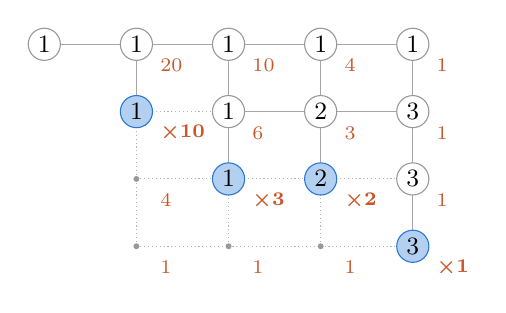
\begin{tikzpicture}[scale=0.9]\pascalstaircase\end{tikzpicture}
\caption{The first-passage identity for $n = 4$ on the counting grid of
Paper~1 (Figure~\ref{P1-fig:grid}): a step right for every \bw{1}, a step down for every \bw{0}. As there, a
white circle holds the number of walks that reach it with the level above $1$ all
the way, and a blue circle is the first point below level $1$ of one Order, reached
by $a(1), \dots, a(4) = 1, 1, 2, 3$ walks. The small numbers count all walks from
a point to the end corner, also along the dotted lines: Pascal's triangle, read from
that corner. Each blue circle times its small number, added up, gives the $20$ below
the first \bw{1}: $1\cdot 10 + 1\cdot 3 + 2\cdot 2 + 3\cdot 1$.}
\label{fig:pascal4}
\end{figure}

\nopagebreak
The same argument works for
other lengths: for every $M \ge m(n-1)$,
\[
\binom{M}{n-1} \;=\; a(n) + \sum_{i=1}^{n-1} a(i)\binom{M - m(i)}{n-i}
\qquad(\text{\lean{choose\_eq\_sum\_admSet\_of\_le}}).
\]
$M = m(n)$ is the identity above; $M = m(n-1)$ gives a recurrence for $a(n)$.
For $n = 5$ and $M = 6$: $a(5) = \binom64 - (5 + 1 + 2 + 0) = 15 - 8 = 7$.
The Lean proof is an induction on $n$ with Pascal's rule in $M$, anchored at
$M = m(n)$.

\subsection*{Counting active words}

Remove from an admissible word of Order $n+1$ its last \bw{1} and the \bw{0}s after
it. What remains is an active word with $n$ ones (Chapter~\ref{sec:words}), and
every active word arises exactly once. So $a(n+1)$ also counts the active words
with $n$ ones (\lean{card\_persSet}; cf.\ Hikawa and Nakanishi~\cite{HikawaNakanishi2026},
Nakanishi~\cite{Nakanishi2026}, Hikawa~\cite{Hikawa2026}). This
is the count computed by K.~Hikawa's Python program linked from OEIS A100982\index{OEIS!A100982}.
Figure~\ref{fig:threecounts} puts the three counts side by side for Order $5$.

\begin{figure}[htbp]
\centering
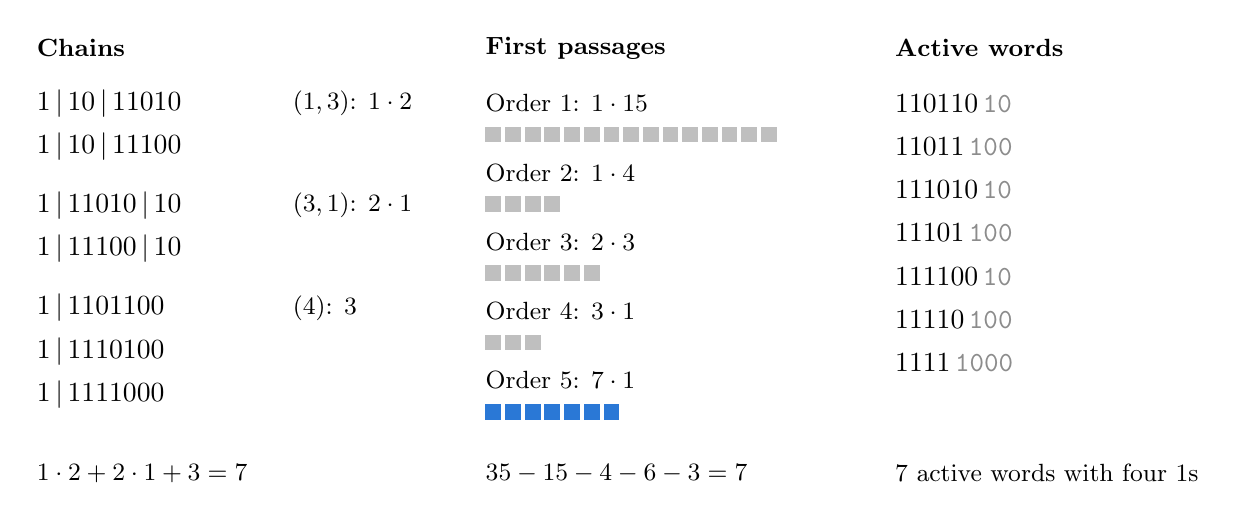
\begin{tikzpicture}\threecounts\end{tikzpicture}
\caption{Three ways to count the $a(5) = 7$ admissible words of Order $5$. Left: their
chains, grouped by the Orders of the blocks. Middle: the $\binom{7}{4} = 35$ words of
length $8$ with five \bw{1}s that start with \bw{1}, one square each, by the Order
of their first passage; the last row is the admissible words themselves. Right: the
active words with four \bw{1}s, each followed in grey by the \bw{1} and the \bw{0}s
that were removed.}
\label{fig:threecounts}
\end{figure}

\subsection*{How big is $a(n)$?}

Winkler~\cite{Winkler2026b} proved
$\frac1n\binom{m(n)-1}{n-1} \le a(n) \le \frac1n\binom{m(n)}{n-1}$,
with equality in the upper bound exactly at the upper record Orders of
Chapter~\ref{sec:chain}, and in the lower bound at the lower record Orders;
there $a(n)$ is a rational Catalan number. For example
$a(5) = 7 = \frac15\binom{7}{4}$.

\subsection*{How often}

Of the positive integers, the fraction $a(n)/2^{p_2(n)}$ lies in a class of Order $n$: $1/4$
for Order $1$, $1/16$ for Order $2$, $2/32$ for Order $3$. If the width
identity of Chapter~\ref{sec:open} holds, this is the fraction whose
dropping time is $p_2(n)$, the pattern recorded in A186008\index{OEIS!A186008}~\cite{OEIS_A186008}.

\begin{wordbox}
\boxhere{mn}$m(n)$\index{m(n)@\termlink{mn}{$m(n)$}|textbf} & $p_2(n) - 1$. \\
\boxhere{composition}composition\index{composition@\termlink{composition}{composition}|textbf} & a list of positive integers with a given sum. \\
A056576\index{OEIS!A056576} & $m(n)$. \\
A186008\index{OEIS!A186008} & class ids by dropping time, as offsets.
\end{wordbox}

%% ======================================================================
\section{The fast map and sorting}
\label{sec:fast}

\termhere{R}A run of odd steps can be done in one go, by the \keyterm{R}{fast map} $R$. If $x$ is odd and ends in $v$ binary
\texttt{1}s, the next $v$ steps are all odd, and with the halving that follows them they give
\[
R(x) = \frac{\tfrac{3^v}{2^v}(x+1) - 1}{2} \qquad (x \text{ odd}),
\qquad R(x) = \frac{x}{2^w} \qquad (x \text{ even}, \ w \text{ trailing \texttt{0}s}).
\]
In binary this is a stack operation: $R$ removes the block $\texttt{0}\,\texttt{1}^v$ from the low
end of $x$, multiplies what remains by $3^v$, and adds the base-$3$ number
$\texttt{11}\cdots\texttt{1}_3$ ($v$ digits).
For example $27 = \bin{11011}$ ends in two \texttt{1}s: $R(27) = (9\cdot 28/4 - 1)/2 = 31$.
After a run of $v$ odd steps from $x$, the number of halvings that follow is
A375782\index{OEIS!A375782}$(x)$~\cite{OEIS_A375782}. Vaillant and Delarue's map~\cite{VaillantDelarue2019}, no ride of $T$ ($13 \mapsto 3$), works on the index $k$ of the odd number $2k+1$
(A324245\index{OEIS!A324245}~\cite{OEIS_A324245}); its change of $k$ is
A349414\index{OEIS!A349414}~\cite{OEIS_A349414}, with one simple formula per residue of $k$
modulo $4$. And for fun: the same split of $x$ at its rightmost
\texttt{0}-bit, into a head and a tail of \texttt{1}s, drives the self-inverse permutation
A387325\index{OEIS!A387325}~\cite{OEIS_A387325}, which swaps the head with the length of the tail.
The split also gives a continued fraction. With the point $1$ for the number $0$, a digit
\texttt{1} below a number takes its point $y$ to $y+1$, a digit \texttt{0} to $1/(y+1)$; so the
point of $x$ is $v + 1/(y+1)$, with $y$ the point of what remains above the \texttt{0} (\lean{markerPoint\_ht}; $v + 1$ if nothing remains):
$2 + 1/(3+1)$ for $27$. Each further run of $v$ \texttt{1}s, with the \texttt{0} below it, is a
quotient $v+1$ (the highest: $v+2$): the $1$-bit markers of the trees of Hanna, Czyz and Self
and of Yu-Ting~\cite{Ryde2020}, with the digits complemented. Read from the highest digit,
the same two maps give the runs in the reverse order: the highest run first, as $v$, the
lowest last, as $v+2$ (\lean{hiPoint\_runs}); and Ryde's two trees carry the two readings at
the complemented node (\lean{aytPoint\_complement}, \lean{hcsPoint\_complement}).

\subsection*{Marked vectors}

\termhere{markedvector}The $R$-trajectory of $x$ up to its drop is recorded as a \keyterm{markedvector}{marked
vector}: an entry $v$ for each run of $v$ odd steps, and an entry $-h$ for each
run of $h$ halvings that $R$ takes from an even value. (The one halving that ends
a run of odd steps is part of that run and is not counted.) The last run of
halvings stops as soon as the value is below the start. For example $1087$ gives
$[6, -2, 1, -1]$ and $1855$ gives $[6, -1, 1, -2]$: the same odd runs, with
different halvings between them (the PARI/GP code of Appendix~\ref{app:pari} prints
them with \texttt{t(x, 1)}). No entry is $0$, and no two negative entries are
neighbours.

\nopagebreak
Read back letter by letter, $v$ \bw{1}s and a \bw{0} for an entry $v$ and $h$
\bw{0}s for an entry $-h$, the marked vector of a start that drops is its word
(\lean{decodeVector\_eq\_tBits}); so its positive entries add up to the Order
(\lean{order\_preservation}). For class ids of one Order above their
cycle point the marked vector determines the class id
(\lean{classId\_eq\_of\_markedVector\_eq}).

\subsection*{Everything sorts alike}
\phantomsection\label{sec:sorting}

Within one Order, sort the class ids (above their cycle points) by their parity
words, or by their marked vectors: the result is the same order
(\lean{tBits\_lt\_iff\_markedVector\_lt}).
The classes can also be generated in this order directly, by a tree that
extends each word by its possible next pieces (\lean{lex\_enumeration}; in PARI/GP,
Appendix~\ref{app:pari}); the
rank of Chapter~\ref{sec:words} is the position in this order.

\nopagebreak
A number sorts the same way. Read a word as a path down the Stern--Brocot tree from $1/1$,
\bw{1} to the right and \bw{0} to the left~\cite{Ryde2020}: its runs (an entry $v$ of the marked
vector, then $1 + h$ \bw{0}s) are the quotients of the continued fraction of the point it
reaches, the last run counted with $1$ more (\lean{sbPoint\_runs}). So $1087$, with runs
$6, 3, 1, 2$, reaches $6 + 1/(3 + 1/(1 + 1/3))$. No admissible word is a prefix of another, so
all of them are sorted like their points (\lean{sbPoint\_lt\_iff\_lt}). The point of a word is
the mediant of the two fractions of its node (\lean{sbPoint\_eq\_sbMed}); the intervals between
those two fractions are disjoint and sorted the same way, and two of them touch exactly when
one word is $v$ followed by \bw{0} and the other $v$ followed by \bw{1} and only \bw{0}s
(\lean{admissible\_touch\_iff}). Every fraction strictly inside the interval of a word is
the point of exactly one word that continues it, so the classes below a word meet the
fractions of its interval one to one (\lean{existsUnique\_class\_point}); once such a word
drops, the fraction lies inside the interval of its drop word
(\lean{exists\_admissible\_between}, \lean{sbNode\_inside}).

\begin{wordbox}
\boxhere{R}$R$\index{R@\termlink{R}{$R$ (fast map)}|textbf} & the fast map: a whole run of odd steps, or all halvings, at once. \\
\boxhere{markedvector}marked vector\index{marked vector@\termlink{markedvector}{marked vector}|textbf} & $R$-trajectory up to the drop: $v$ per odd run, $-h$ per
  run of $h$ halvings. \\
A375782, A349414\index{OEIS!A375782}\index{OEIS!A349414} & halvings after an odd run; index change under A324245. \\
A324245\index{OEIS!A324245} & the map of Vaillant and Delarue on the index $k$ of $2k+1$. \\
A387325\index{OEIS!A387325} & head/tail-length swap around the rightmost \texttt{0}-bit.
\end{wordbox}

%% ======================================================================
\section{What is still open}
\label{sec:open}

The question ``does every $x > 1$ drop?'' splits into two precise parts.
\termhere{cst}Recall that the level of $x$'s parity word is a product of $3/2$s and $1/2$s;
the \keyterm{cst}{coefficient stopping time} of $x$ is the length of the first prefix
of its parity word whose level is below $1$, if there is one.

\begin{itemize}
\item\phantomsection\label{conj:covering} \termhere{covering}\keyterm{covering}{Covering.} Every $x > 1$ has a coefficient stopping time, that
  is, some prefix of its parity word is admissible (Lean: \lean{Covering}).
\item\phantomsection\label{conj:width} \termhere{widthidentity}\keyterm{widthidentity}{Width identity} (Terras~\cite{Terras1976}, Conjecture~2.9).
  Every $x > 1$ drops exactly at its coefficient stopping time
  (\lean{WidthIdentity}). Equivalently: every class id above $1$ lies above its
  cycle point of Chapter~\ref{sec:numbers} (\lean{ClassDrops},
  \lean{widthIdentity\_iff\_classDrops}). Appendix~\ref{app:width} says why it is
  hard.
\end{itemize}
If every $x > 1$ drops, every $x > 1$ has a coefficient stopping time
(\lean{covering\_of\_drops}), and the two parts together give the drop for every
$x > 1$ (\lean{drops\_of\_covering\_width}; for the fast map,
\lean{drop\_of\_covering\_width}), hence, by Chapter~\ref{sec:intro}, the classic
conjecture.

\nopagebreak
The width identity would settle another question on the way: it leaves no room
for a cycle. On a cycle the smallest value $y$ comes back to itself, so the level
of its parity word falls below $1$ within one round, while no value on the cycle
is below $y$. That is a failure of the width identity. So if the width
identity holds, the only cycle of $T$ is $1 \to 2 \to 1$
(\lean{no\_cycle\_of\_widthIdentity}). No other cycle is known, but proving that
there is none is itself an open problem.

\subsection*{The drop as termination}

The drop question is a termination question, and nothing in it looks past the
drop. Fix a start $s$ and allow a step $x \mapsto f(x)$ only while $x \ge s$:
a value below $s$ is final. This rewriting from $s$ terminates exactly when $s$
drops (\lean{DescendToMinimum.acc\_iff\_drops}, for any map $f$). So the drop conjecture says:
from every start $s > 1$, the rewriting with the fast map $R$ terminates
(\lean{dropConjecture\_iff\_acc}). A proof along this line needs a measure that
goes down at every allowed step, the rising ones included; none is known.

\subsection*{Evidence}

All class ids of Orders $2$ to $15$ lie above their cycle points, with ratio
$q \le 251/507$ (\pv{maxq 2 \dots\ 15}); among the class ids below $20\,000\,000$ the tightest case is
$x = 47$ at Order $34$.
A direct check of every class of Orders $2$ to $30$ (a C++ program) confirms that all class ids
drop, and that in each of these Orders the smallest difference between class id
and drop value occurs at the smallest class id.
The fraction of positive integers not yet covered by admissible classes of
Order at most $n$ is the fraction of active words among all words of length
$p_2(n)$, that is $\mathrm{A076227}\index{OEIS!A076227}(p_2(n))/2^{p_2(n)}$: $1/2, 1/4, 3/16, 1/8, 13/128,
19/256, 1/16, \dots$ for $n = 0, 1, 2, \dots$. By Terras~\cite{Terras1976} it shrinks towards $0$; since
all but finitely many members of a class drop, almost all $x$ drop. Where the width identity holds, the smallest $x > 1$ not yet covered
is $2, 3, 7, 27, 703, 10087, 35655, \dots$ (OEIS A060412\index{OEIS!A060412}~\cite{OEIS_A060412}): each has a larger Order
than every smaller start, and gives way to the next at its own Order,
$0, 2, 4, 37, 51, 66, 85, \dots$

\subsection*{A finite check for the width identity}

The number $\rho$ of a word cannot be large. An odd step with $k$ letters before it adds
$3^{n-o}\,2^k$ to $\rho$, where $n$ is the Order and $o$ counts the odd steps up to
and including position $k$. Before that step the level of an admissible word is
at least $1$, so $2^k \le 3^{o-1}$, and each odd step adds at most $3^{n-1}$. Hence
$\rho \le n\,3^{n-1}$ for every admissible word of Order $n$
(\lean{rho\_le\_of\_admissible}). The largest $\rho$ comes from the first word alone
(\lean{rho\_eq\_rhoMax\_iff}); twice what it leaves of $n\,3^{n-1}$ is the sum of the terms
$3^{n-1-m}(2 \cdot 3^m - 2^{p_2(m)})$ over $m < n$ (\lean{rhoMax\_slack}), and the term of $m$
is below every earlier one from $1$ on exactly at the lower record Orders
(\lean{lowerRecord\_iff\_slackTerm}). From below, $\rho \ge 3^n - 2^n$ for every word of
Order $n$, with equality exactly for the words that start with all their odd steps
(\lean{three\_pow\_le\_rho\_add}, \lean{rho\_add\_eq\_three\_pow\_iff}). \termhere{tau}By the drop test of Chapter~\ref{sec:numbers},
every member $x$ with $n\,3^{n-1} < d_{23}\,x$ drops at the end of its word
(\lean{drop\_of\_large}). As $p_2$ depends only on the Order, so does $d_{23}$,
and the width identity only needs checking at class ids up to
\[
\keysym{tau}{\tau(n)} = \frac{n\,3^{n-1}}{d_{23}(n)}
\]
(\lean{classDrops\_iff\_small}). This bound is small unless $2^{p_2(n)}$ comes
very close to $3^n$. It is above its value at every earlier Order exactly at the
upper record Orders of the block factor of Chapter~\ref{sec:chain}, and so is
$\lfloor \tau(n) \rfloor$ (\lean{upperRecord\_iff\_tau},
\lean{upperRecord\_iff\_widthBound}). The reason: let $n$ be no upper record Order, $a$
the last upper record Order below it and $m = n - a$. Then $p_2(n) = p_2(a) + p_2(m)$,
and $\tau(m) \le \tau(a)$, by induction, gives $\tau(n) < \tau(a)$ (\lean{tau\_add\_lt}). There are
$37$ of these Orders up to $2\cdot 10^6$; some of them are in Table~\ref{tab:tau},
beside the walk that finds them (Figure~\ref{fig:tau}).

\begin{figure}[htbp]
\centering
\begin{minipage}[c]{0.4\linewidth}\centering
\makeatletter\def\@captype{table}\makeatother
$\begin{array}{r r}
\toprule
n & \lfloor \tau(n) \rfloor \\
\midrule
17 & 144 \\
41 & 1\,185 \\
306 & 99\,729 \\
15\,601 & 285\,814\,986 \\
47\,468 & 1\,447\,674\,321 \\
79\,335 & 7\,216\,089\,270 \\
190\,537 & 984\,572\,779\,224 \\
\bottomrule
\end{array}$
\caption{Some records of $\lfloor \tau(n) \rfloor$.}
\label{tab:tau}
\end{minipage}\hfill
\begin{minipage}[c]{0.55\linewidth}\centering
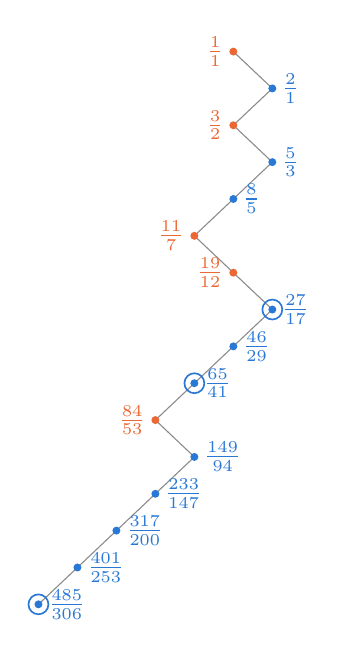
\begin{tikzpicture}[scale=0.9]\sternbrocotpath\end{tikzpicture}
\caption{The walk down the Stern--Brocot tree towards $\log_2 3$
(Chapter~\ref{sec:chain}); blue fractions lie above $\log_2 3$, orange ones below, and
every blue denominator is a record Order of $\tau$; those of Table~\ref{tab:tau} are
ringed.}
\label{fig:tau}
\end{minipage}
\end{figure}

The last of them is $190\,537$ and the next $10\,781\,274$ (by the walk, computed by Lean's
kernel), so
$\lfloor \tau(n) \rfloor$ is largest at $190\,537$ for $n < 10\,781\,274$
(\lean{widthBound\_le\_of\_upperRecord}). A C++ program,
also outside Lean, checked that every $x$ with $1 < x \le 984\,572\,779\,224$ drops at its
coefficient stopping time; the largest Order met is $347$ (at $x = 898\,696\,369\,947$).

So the width identity holds for every admissible word of Order at most $10\,781\,273$:
a computer-assisted result, since the range check enters the Lean proof as its only
hypothesis (\lean{classDropsAt\_le\_10781273}). An independent residue-class sieve and a
second run of the program on other hardware reproduced the range check. The step to the
Orders is formal too: if every $x$ with
$1 < x \le X$ drops at its coefficient stopping time, the width identity holds at
every Order $n$ with $\lfloor \tau(n) \rfloor \le X$
(\lean{classDropsAt\_of\_verified}); with the records of $\tau$, at every Order up to
$n$ as soon as $X$ reaches $\lfloor \tau \rfloor$ of the last upper record Order up to
$n$ (\lean{classDropsAt\_of\_verified\_record}).

How large can $\tau(n)$ get? Rhin~\cite[Proposition, p.~160, (7)]{Rhin1987} proved
that $|u_0 + u_1 \log 2 + u_2 \log 3| \ge H^{-13.3}$ for integers $u_0, u_1, u_2$ with
$H = \max(|u_1|, |u_2|) \ge 2$ (natural logarithms). With $u_0 = 0$, $u_1 = p_2(n)$,
$u_2 = -n$ this gives
$2^{p_2(n)} - 3^n \ge 3^n\,p_2(n)^{-13.3}$, so $\tau(n) \le n\,p_2(n)^{13.3}/3$:
the class ids to check grow at most polynomially with the Order. Mintz's exact
count of the $3$-smooth numbers uses the round-ups $p_2(k)$ of $k\log_2 3$; Rhin's bound says
how small their excess can get. (Cited, not formalized: with $u_0 = 0$ it is the hypothesis \lean{RhinLog}; his proof
of (7) uses a computation by E.~Dubois and P.~Toffin.)
Under the hypothesis $3^n \le K\,p_2(n)^C\,(2^{p_2(n)} - 3^n)$ for every $n \ge 1$
(\lean{RhinBound}; Rhin's bound gives $K = 1$, $C = 14$: \lean{rhinBound\_of\_rhinLog}), the width identity at
Order $n$ follows once every $x$ with $1 < x \le K\,2^C n^{C+1}$ whose word has
Order $n$ is checked to drop at its coefficient stopping time
(\lean{classDropsAt\_of\_rhinBound}; for all Orders together,
\lean{classDrops\_of\_rhinBound}). Exceptions at finitely many Orders only raise
$K$ (\lean{rhinBound\_of\_rhinBoundFrom}). Lean's kernel checks that $K = 1$ and
$C = 2$ suffice for every $n \le 10^{60}$ (\lean{rhinBoundUpTo\_one\_two}); no proof uses it.

\subsection*{Two kinds of question}

Which class $x$ belongs to depends only on its lowest binary digits: a $2$-adic
question, blind to size. Whether $x$ drops depends on its size. Inside one class
the two agree, above the cycle point (Chapter~\ref{sec:numbers}); across all
classes they are the covering question. This tension, $2$-adic dynamics against
an ordinary size condition, runs through the whole problem~\cite{Lagarias1985}.
It also separates the fractions above from Terras's theorem~\cite{Terras1976}
that almost all $x$ drop: ours are exact finite fractions, not asymptotic
densities.

\subsection*{Side results}

\emph{Minimal class ids.} The smallest class id of each Order is OEIS
A122442\index{OEIS!A122442}~\cite{OEIS_A122442} (Chapter~\ref{sec:numbers}). Ten of the smallest class ids, those of Orders $37$, $35$, $34$, $32$, $28$, $26$,
$25$, $18$, $17$ and $15$, lie on one way to a drop, the one of $27$: $27$, $31$, $47$,
$71$, $91$, $103$, $155$, $167$, $251$ and $283$ all wait for the same long way down.

\emph{Mersenne starts.} For odd $k \ge 5$, if $2^k - 1$ and $2^{k+1} - 1$ both drop, the first has at least
the Order of the second: both reach $(3^{k+1} - 1)/8$ after $k + 1$ odd steps and then share
their way down, where the larger start drops no later
(\lean{order\_mersenne\_succ\_le}).

\emph{Only $3 \bmod 4$ matters.}\phantomsection\label{sec:mod4} Every class id of Order $\ge 2$ is
$3 \bmod 4$: even numbers drop in one step, and $4i+1$ in two
(Chapter~\ref{sec:intro}; \lean{classId\_mod4}, \lean{order\_trichotomy}).

\emph{From $3 \bmod 4$ to $3 \bmod 4$.} So take a value $x$ that is $3 \bmod 4$, with
$x + 1 = 2^v s$ and $s$ odd. It takes $v$ odd steps, up to $3^v s - 1$; a
\emph{G-step} goes on from there to the next value that is $3 \bmod 4$, or below the
start (\lean{gStep\_spec}, \lean{gStep\_formula}). The first value below the start is
its drop, and a start drops exactly when its chain of G-steps gets there
(\lean{gChain\_drop}, \lean{gChain\_drop\_iff}). The numbers of G-steps to the drops of
$3, 7, 11, 15, \dots$ are A400742\index{OEIS!A400742}~\cite{OEIS_A400742}; for $27$
there are $9$.

\nopagebreak
\emph{Looking backwards.} For $m > 1$ not divisible by $3$, some odd number above
$m$ passes through $m$, and so drops. With $3x+1$ and the halving after it counted as
two steps, the smallest one is A350082\index{OEIS!A350082}$(m)$~\cite{OEIS_A350082};
$T$ skips the values $3x+1$, so under $T$ it can be larger ($21$, not $17$, for $m = 16$).

\begin{wordbox}
\boxhere{cst}coefficient stopping time\index{coefficient stopping time@\termlink{cst}{coefficient stopping time}|textbf} & length of the first prefix of $x$'s parity word
  with level below $1$. \\
\boxhere{covering}Covering\index{covering@\termlink{covering}{Covering}|textbf} & every $x > 1$ has a coefficient stopping time. \\
\boxhere{widthidentity}Width identity\index{width identity@\termlink{widthidentity}{Width identity}|textbf} & every $x > 1$ drops at its coefficient stopping time
  (Terras 1976, Conj.~2.9). \\
\boxhere{tau}$\tau(n)$\index{tau(n)@\termlink{tau}{$\tau(n)$}|textbf} & $n\,3^{n-1}/d_{23}$; class ids above it drop at the end of their
  word. \\
A060412\index{OEIS!A060412} & smallest integers not yet covered; each has a larger Order than every smaller start. \\
A350082\index{OEIS!A350082} & smallest larger odd number passing through $m$, with $3x+1$ as a step of its own. \\
A400742\index{OEIS!A400742} & G-steps to the drop of $4n+3$.
\end{wordbox}

%% ======================================================================
\appendix

\section{The Lean formalization}
\label{app:lean}

The Lean~4 project \lean{AcceleratedCollatz} (Mathlib) proves every result
that this paper cites with a Lean name, without \texttt{sorry}; open statements and
theorems taken from the literature enter as named hypotheses. A self-contained file
\texttt{ChainDecomposition.lean} holds the admissible words, the chain
decomposition with its budget and record lows, the count by chains and the two
binomial identities, with Mathlib as its only dependency. A second one,
\texttt{SweepQ.lean}, holds the sweep, the start sweep and the cut sweep for the
words of every odd $q \ge 3$. A third, \texttt{ChainQ.lean}, holds their chain
decomposition with its codes, count and budget, the gaps of the record Orders and the
first word of each Order. A fourth, \texttt{SmoothPlace.lean}, holds the place of
$p^a q^b$ among the numbers $p^i q^j$ for any two bases. A fifth,
\texttt{SmoothRuler.lean}, also with Mathlib only, is built with the project through
\lean{TRulerRecord}; it holds an open statement on neighbouring $3$-smooth numbers that
this paper does not use.

\subsection*{How this was made}

The Lean files, the scripts and this text were written in conversation with
Claude (Anthropic); M.~Winkler worked with ChatGPT (OpenAI). Ideas were tried numerically first, then stated and proved in
Lean, compiled locally, and every open end was logged for the next session. Some
of it went better than planned. Once the words were cut at their record lows, the
blocks turned out to be admissible words again, with a condition on their Orders
only; the proofs of Chapters~\ref{sec:chain} and~\ref{sec:count} then became short
and clean. An independent audit, commissioned by M.~Winkler, compiled an earlier
version of \texttt{ChainDecomposition.lean} and checked its proofs once more with a second
checker. The same workflow is open to any reader:
the Lean proofs can be checked on any computer, and \texttt{pv.py} reproduces the
examples. Table~\ref{tab:lean} lists the lean-files.

\begin{table}[p]
\centering
\footnotesize
\begin{tabular}{@{}>{\raggedright\arraybackslash}p{0.42\linewidth}>{\raggedright\arraybackslash}p{0.5\linewidth}@{}}
\toprule
lean-file & content \\
\midrule
\lean{DescendToMinimum}, \lean{DropEquivalence$\{$,T$\}$}, \lean{DropTermination}
  & drop conjecture $\iff$ classic conjecture; the drop as termination \\
\lean{Numlib}
  & general number theory \\
\lean{AdmissibleLength}, \lean{TStaircase}
  & admissible words, length $p_2$, prefix property, step bound \\
\lean{TParity}, \lean{TRho$\{$Lower,Max,Slack$\}$}
  & the step $T$, parity words, $\rho$ and its least and largest values, the terms of its slack, $d_{23}$ \\
\lean{TAffine}, \lean{TClass}, \lean{TCongruenceSplit}, \lean{TCorrespondence}, \lean{TDrop}
  & drop test and cycle point, classes and their marked vectors, class ids, drop formula, the bound of a split \\
\lean{TMod4}, \lean{TSieve}
  & Collatz-primes; only $3 \bmod 4$ matters \\
\lean{TBridge}, \lean{TEncode}, \lean{TFold}
  & encodings and cores; folds and $\rho$; marked vectors and parity words \\
\lean{TBudget}, \lean{TChain$\{$,Orders$\}$}, \lean{TFirst$\{$Greedy,Orders,Word$\}$}, \lean{TRecordLow}, \lean{TSplit$\{$,Grammar$\}$}
  & first-drop parse, chain decomposition, Order-only validity, budget, record lows, the first word of each Order, also as a greedy sum \\
\lean{TAttrs}, \lean{TChain$\{$Equiv,Parse$\}$}
  & chains and codes as bijections, their computable form, all attributes of an odd part \\
\lean{TActive}, \lean{TAdmSet}, \lean{TBinomial$\{$,Range$\}$}, \lean{TCount}, \lean{TPersistent}
  & the counts of Chapters~\ref{sec:words} and~\ref{sec:count} \\
\lean{TPrefixCount}, \lean{TRank}
  & counting by prefix, rank and unrank \\
\lean{Core}, \lean{MarkedVector$\{$,Shift$\}$}, \lean{OrderPreservation}, \lean{R$\{$Map,Shift$\}$}, \lean{TMarker$\{$Point,PointHigh,Tree$\}$}
  & fast map, shifts by multiples of a large power of $2$, marked vectors, the point of a number \\
\lean{TLex}, \lean{TSternBrocot$\{$Interval,Onto,Tree$\}$}, \lean{Tree}, \lean{TVectorLex}, \lean{TWordPoint}
  & tree construction, sorting, the point of a word, also as a mediant, the intervals of the words, every positive rational reached once \\
\lean{TRLink}
  & the drop under $R$ and under $T$ \\
\lean{TCovering}, \lean{TCycle}, \lean{TFiniteCheck}, \lean{TRhin$\{$Bound,Check,Log$\}$}, \lean{TRho$\{$Bound,Max$\{$Bound,Check,Record$\}\}$}, \lean{TRuler$\{$Check,Pair$\}$}, \lean{TWidth$\{$,Bound,Record$\}$}
  & the open parts of Chapter~\ref{sec:open}, the finite check and the records of $\tau$ and of the largest $\rho$ over $d_{23}$, the bound from Rhin, no cycles under the width identity \\
\lean{TBracket$\{$,Chain,Decode,Dyck,Parse,Tree$\}\{$,Q$\}$}, \lean{TBracket$\{$Count,Drop$\}$}, \lean{TBracket$\{$Clash,One,WordTree$\}$Q}, \lean{TNest}
  & first drops, brackets, bracket words, bracket trees, their decoder and count; bracket words, their chain form, trees, tree parser and decoder, one-bracket words, for every $q \ge 3$ \\
\lean{SmoothRuler}, \lean{TBlockRecord}, \lean{TGridOrder}, \lean{TRuler$\{$Deficit,Record$\}$}, \lean{TSmooth$\{$Between,Class,Next,Place,Succ$\}$}, \lean{TStartSweep}, \lean{TSternBrocot$\{$,Conv$\}$}, \lean{TSweep$\{$,Perm,Z$\}$}
  & the sweep map, the start and cut sweeps, record Orders as linear grids, by the block factor, on the Stern--Brocot walk and as the semiconvergents of $\log_2 3$, the $3$-smooth numbers in order, each the upper or the lower step of the one before, and by their number of binary digits; the integer sweep, Thomas--Williams as hypothesis \\
\lean{TBisect}, \lean{TFloorSum}, \lean{TRecord$\{$Floor,Walk$\}$}, \lean{TSmooth$\{$Program,ProgramConv,Rank$\}$}, \lean{TSternBrocotCert}
  & the A003586 program: floor sums, bisections, the walk to the last record Orders, the $n$-th $3$-smooth number from a convergent of $\log_2 3$, also by the Stern--Brocot walk in integers, for every $n$ \\
\lean{TBudgetQ}, \lean{TChain$\{$,Equiv$\}$Q}, \lean{TCountQ}, \lean{TFirst$\{$Chain,Greedy,Orders,Word$\}$Q}, \lean{TRecordLowQ}, \lean{TSplitQ}, \lean{TWordQ}
  & the chain decomposition with its codes, count and budget, record lows, the first word, for the words of every odd $q \ge 3$ \\
\lean{TBlockRecordQ}, \lean{TCutSweepQ}, \lean{TGridOrderQ}, \lean{TLastRecordsQ}, \lean{TRecordGapQ}, \lean{TSmooth$\{$Class,Next,Place,Succ$\}$Q}, \lean{TStartSweep$\{$,Inj,Perm$\}$Q}, \lean{TSternBrocot$\{$,Conv$\}$Q}, \lean{TSweep$\{$,Perm$\}$Q}
  & the sweeps and the record Orders, also on the Stern--Brocot walk and as semiconvergents, for every odd $q \ge 3$; the numbers $2^j q^i$ in order \\
\lean{TGMap}, \lean{TMersenne}
  & steps from $3 \bmod 4$ to $3 \bmod 4$, Mersenne starts \\
\lean{DeadCode}
  & unused declarations, not imported by the library \\
\bottomrule
\end{tabular}
\caption{The lean-files: all $144$, and \lean{DeadCode}; braces group names as in a shell, so \lean{TWidth$\{$,Bound$\}$} is \lean{TWidth} and \lean{TWidthBound}.}
\label{tab:lean}
\end{table}

\section{PARI/GP}
\label{app:pari}

The tree construction lists all classes up to Order $N$, as in
Paper~1, Appendix~\ref{P1-app:table}; the map and trajectory code computes the $R$-trajectory,
Order and marked vector of any start.

\begin{lstlisting}[basicstyle=\ttfamily\scriptsize, breaklines=true]
\\ Tree construction: all admissible classes up to Order N,
\\ as rows [encoding, rho, class id, p2, drop, p3]
\\ q3: the powers 3^0 .. 3^N; p2: their bit lengths; r: the rows of one Order.
\\ A row with encoding s has one child per trailing 0 of s (the root has one);
\\ child i of a row with p2 = u has rho 3 rho + 2^(u - i).
a_iter_R(N) = {
  my( t=1/3, q3=vector(N+1, i, t*=3), p2=[logint(x, 2)+1 | x<-q3]
    , r=[[0, 0, 2, 1, 1, 0]]
    );
  concat(concat([r], vector(N, n
  , my( q=q3[n+1], u=p2[n], w=p2[n+1] );
    r= concat(apply(v ->
        my( s=v[1] );
        vector(if(s, valuation(s, 2), 1), i
        , my( rho=3*v[2]+(1<<(u-i)), c=lift(Mod(-rho, 1<<w)/q) );
          [(s+(1<<(i-1)))<<(w-u), rho, c, w, (c*q+rho)>>w, n]
        )
      , r))
  )));
}
\end{lstlisting}

\begin{lstlisting}[basicstyle=\ttfamily\scriptsize, breaklines=true]
\\ Map. m=0: bare display (default, 0 for a run of halvings);
\\ m=1: marked display (-w for a run of w halvings)
{ R(x, m=0) =
  my(p=x%2, w=valuation(x+p,2));
  [ if(p, w, m, -w, 0)
  , if(p, (3^w/2^w*(x+1)-1)/2, x/2^w)
  ];
}

\\ [p2, Order], vector of the steps, trajectory of x up to its drop; drop(1) = 1
{ t(x, m=0) =
  my(h, u=0, p=List(), v=List(x), x0=x);
  until(x < x0 || x == 1
  , [h,x]=R(x,m);
    listput(~p,h); listput(~v,x)
  );
  while(x && x*2 < x0, x*=2; u++);
  if(m, #p && p[#p] < 0 && p[#p]+=u);
  p=Vec(p); v=Vec(v); v[#v]=x;
  my( p3=vecsum([e|e<-p,e>0])
  , p2=logint(3^p3,2)+1
  );
  [[p2, p3], p, v];
}

\\ Test: bare (m=0, default)
? t(27)
% =
[ [59, 37]
, [2, 5, 1, 2, 3, 4, 1, 0, 3, 2, 6, 0, 4, 0, 1, 1, 1, 0, 1, 0]
, [27, 31, 121, 91, 103, 175, 445, 334, 167, 283, 319, 1822, 911, 2308, 577, 433, 325, 244, 61, 46, 23]
]
\\ Test: marked (m=1), the marked vector of the fast-map chapter
? t(27, 1)
% =
[ [59, 37]
, [2, 5, 1, 2, 3, 4, 1, -1, 3, 2, 6, -1, 4, -2, 1, 1, 1, -2, 1, -1]
, [27, 31, 121, 91, 103, 175, 445, 334, 167, 283, 319, 1822, 911, 2308, 577, 433, 325, 244, 61, 46, 23]
]
\end{lstlisting}


\section{Why the width identity is hard}
\label{app:width}

Follow a number $x > 1$ step by step. At every moment its value is the
\emph{idealized} value, the start times the level, plus an extra part that
comes from all the $+1$s so far. That extra part is never negative, and it
changes in a known way: a halving takes it from $e$ to $e/2$, an odd step to
$(3e+1)/2$.

Now keep a reserve: the number of halvings it would take to bring the level
below $1$. An odd step adds one to the reserve or leaves it as it is; each
halving spends one. When the reserve is spent, the idealized value is below the
start. The width identity says that the real value is below the start at that same
step, for the first time. The margin can be thin: for $x = 31$ the two halvings
from $244$ to $61$ leave a reserve of exactly one.

\nopagebreak
Why is this hard to prove? Everything we learn from ``$x$ has not dropped yet''
says that the extra part is not too \emph{small}. To have the real value below the
start when the reserve is spent, we would need to know that it is not too
\emph{large}, and that would have to come from the way the extra part itself changes. Nobody knows how to get
that. This is Terras's Conjecture~2.9~\cite{Terras1976}; Winkler writes it
as $\sigma^* = \sigma$ and leaves it open~\cite{Winkler2017}. The same identity would already rule out
cycles (Chapter~\ref{sec:open}).

\begin{thebibliography}{99}
\bibitem{ALW2014} D.~Armstrong, N.~A. Loehr, and G.~S. Warrington, \emph{Rational
  parking functions and Catalan numbers}, arXiv:1403.1845 (2014).
\bibitem{ALW2015} D.~Armstrong, N.~A. Loehr, and G.~S. Warrington, \emph{Sweep maps:
  a continuous family of sorting algorithms}, Adv.\ Math.\ \textbf{284} (2015), 159--185.
\bibitem{Feller1971} W.~Feller, \emph{An Introduction to Probability Theory and
  Its Applications}, Vol.~II, 2nd ed., Wiley, 1971, Chapter~XII.
\bibitem{GKP1989} R.~L. Graham, D.~E. Knuth, O.~Patashnik, \emph{Concrete
  Mathematics}, Addison-Wesley, Reading, MA, 1989 (6th printing, 1990).
\bibitem{Hikawa2026} K.~Hikawa, \emph{Finite parity-vector structures in the
  accelerated Collatz map}, Kanazawa Gakuin Univ., ResearchGate preprint, 2026,
  \url{https://doi.org/10.13140/RG.2.2.24486.28480}.
\bibitem{HikawaNakanishi2026} K.~Hikawa and K.~Nakanishi, \emph{Parity vector
  analysis in the study of the Collatz conjecture}, ResearchGate preprint,
  January 2026, \url{https://doi.org/10.13140/RG.2.2.12065.06240}.
\bibitem{deWeger2012} T.~Laarhoven and B.~M.~M. de Weger, \emph{The Collatz
  conjecture and De Bruijn graphs}, Indag.\ Math.\ \textbf{24} (2013), 971--983;
  arXiv:1209.3495.
\bibitem{Lagarias1985} J.~C. Lagarias, \emph{The $3x+1$ problem and its
  generalizations}, Amer.\ Math.\ Monthly \textbf{92} (1985), 3--23.
\bibitem{Mintz1981} D.~J. Mintz, \emph{2,3 sequence as binary mixture}, Fibonacci
  Quart.\ \textbf{19} (1981), 351--360.
\bibitem{Nakanishi2026} K.~Nakanishi, \emph{A structural study of parity
  vectors in the Collatz conjecture}, Jxiv preprint, February 2026,
  \url{https://doi.org/10.51094/jxiv.3096}.
\bibitem{OEIS_A000265} OEIS Foundation Inc., \emph{Sequence A000265},
  \url{https://oeis.org/A000265}.
\bibitem{OEIS_A003586} OEIS Foundation Inc., \emph{Sequence A003586},
  \url{https://oeis.org/A003586}.
\bibitem{OEIS_A014682} OEIS Foundation Inc., \emph{Sequence A014682},
  \url{https://oeis.org/A014682}.
\bibitem{OEIS_A020914} OEIS Foundation Inc., \emph{Sequence A020914},
  \url{https://oeis.org/A020914}.
\bibitem{OEIS_A022921} OEIS Foundation Inc., \emph{Sequence A022921},
  \url{https://oeis.org/A022921}.
\bibitem{OEIS_A056576} OEIS Foundation Inc., \emph{Sequence A056576},
  \url{https://oeis.org/A056576}.
\bibitem{OEIS_A060412} OEIS Foundation Inc., \emph{Sequence A060412},
  \url{https://oeis.org/A060412}.
\bibitem{OEIS_A076227} OEIS Foundation Inc., \emph{Sequence A076227},
  \url{https://oeis.org/A076227}.
\bibitem{OEIS_A100982} OEIS Foundation Inc., \emph{Sequence A100982},
  \url{https://oeis.org/A100982}.
\bibitem{OEIS_A122442} OEIS Foundation Inc., \emph{Sequence A122442},
  \url{https://oeis.org/A122442}.
\bibitem{OEIS_A177789} OEIS Foundation Inc., \emph{Sequence A177789},
  \url{https://oeis.org/A177789}.
\bibitem{OEIS_A186008} OEIS Foundation Inc., \emph{Sequence A186008},
  \url{https://oeis.org/A186008}.
\bibitem{OEIS_A206788} OEIS Foundation Inc., \emph{Sequence A206788},
  \url{https://oeis.org/A206788}.
\bibitem{OEIS_A243115} OEIS Foundation Inc., \emph{Sequence A243115},
  \url{https://oeis.org/A243115}.
\bibitem{OEIS_A260591} OEIS Foundation Inc., \emph{Sequence A260591},
  \url{https://oeis.org/A260591}.
\bibitem{OEIS_A324245} OEIS Foundation Inc., \emph{Sequence A324245},
  \url{https://oeis.org/A324245}.
\bibitem{OEIS_A349414} OEIS Foundation Inc., \emph{Sequence A349414},
  \url{https://oeis.org/A349414}.
\bibitem{OEIS_A350082} OEIS Foundation Inc., \emph{Sequence A350082},
  \url{https://oeis.org/A350082}.
\bibitem{OEIS_A368514} OEIS Foundation Inc., \emph{Sequence A368514},
  \url{https://oeis.org/A368514}.
\bibitem{OEIS_A375782} OEIS Foundation Inc., \emph{Sequence A375782},
  \url{https://oeis.org/A375782}.
\bibitem{OEIS_A375961} OEIS Foundation Inc., \emph{Sequence A375961},
  \url{https://oeis.org/A375961}.
\bibitem{OEIS_A387325} OEIS Foundation Inc., \emph{Sequence A387325},
  \url{https://oeis.org/A387325}.
\bibitem{OEIS_A400742} OEIS Foundation Inc., \emph{Sequence A400742},
  \url{https://oeis.org/A400742}.
\bibitem{Rhin1987} G.~Rhin, \emph{Approximants de Pad\'e et mesures effectives
  d'irrationalit\'e}, S\'eminaire de Th\'eorie des Nombres, Paris 1985--86,
  Progr.\ Math.\ 71, Birkh\"auser, Boston, 1987, 155--164.
\bibitem{Ryde2020} K.~Ryde, \emph{Trees of Rationals}, draft (2020),
  \url{https://user42.tuxfamily.org/rationals/index.html}.
\bibitem{Terras1976} R.~Terras, \emph{A stopping time problem on the positive
  integers}, Acta Arith.\ \textbf{30} (1976), 241--252.
\bibitem{ThomasWilliams2018} H.~Thomas and N.~Williams, \emph{Sweeping up zeta},
  Selecta Math.\ \textbf{24} (2018), 2003--2034, doi:10.1007/s00029-018-0408-0,
  arXiv:1512.01483v5 [math.CO] 27 Feb 2018.
\bibitem{VaillantDelarue2019} N.~Vaillant and P.~Delarue, \emph{The hidden face of the
  $3x+1$ problem. Part I: Intrinsic algorithm} (2019); linked from OEIS A324245.
\bibitem{Paper1} Ruud H.G. van Tol, \emph{Collatz, but stop at the drop; Now with less noise}
  (2026).
\bibitem{Winkler2017} M.~Winkler, \emph{Deterministic structures in the
  coefficient stopping-time dynamics of the $3x+1$ problem}, arXiv:1709.03385v8 (2026).
\bibitem{Winkler2026a} M.~Winkler, \emph{Coefficient first-passage words for
  the $3x+1$ map: a Beatty--Ferrers model and a power-of-two law}, preprint,
  September 2026, \url{https://doi.org/10.13140/RG.2.2.31257.79200}.
\bibitem{Winkler2026b} M.~Winkler, \emph{Admissible $qx+1$ sequences,
  semiconvergents, and rational Catalan numbers}, arXiv:2609.22303 (2026).
\end{thebibliography}

\printindex

\end{document}
